\documentclass[aspectratio=169,10pt]{beamer}

% Nueva presentación orientada a resultados finales.
% Fuente de verdad interna: artefactos 03_07/03_07a del 15-08-2026.
\usepackage[utf8]{inputenc}
\usepackage[T1]{fontenc}
\usepackage{lmodern}
\usepackage[spanish,es-nodecimaldot]{babel}
\usepackage{booktabs}
\usepackage{array}
\usepackage{tabularx}
\usepackage{colortbl}
\usepackage{graphicx}
\usepackage{xcolor}
\usepackage{tikz}
\usepackage{pgfplots}
\usepackage{amsmath}
\usepackage{cite}
\usetikzlibrary{arrows.meta,positioning,calc,fit,backgrounds,shapes.geometric}
\pgfplotsset{compat=1.18}

\usetheme{default}
\usefonttheme{professionalfonts}
\setbeamertemplate{navigation symbols}{}

\definecolor{Navy}{HTML}{12304A}
\definecolor{Blue}{HTML}{276FBF}
\definecolor{Teal}{HTML}{148A8A}
\definecolor{Coral}{HTML}{D95D4F}
\definecolor{Gold}{HTML}{D79A22}
\definecolor{Purple}{HTML}{7857A4}
\definecolor{Green}{HTML}{1C8C5E}
\definecolor{Ink}{HTML}{23313D}
\definecolor{Muted}{HTML}{61717E}
\definecolor{Line}{HTML}{D7E0E7}
\definecolor{SoftBlue}{HTML}{EAF2FA}

\setbeamercolor{normal text}{fg=Ink,bg=white}
\setbeamercolor{structure}{fg=Blue}
\setbeamercolor{frametitle}{fg=Navy,bg=white}
\setbeamercolor{title}{fg=Navy}
\setbeamercolor{subtitle}{fg=Muted}
\setbeamercolor{footline}{fg=Muted,bg=white}
\setbeamercolor{block body}{fg=Ink,bg=SoftBlue}
\setbeamercolor{block title}{fg=Navy,bg=Blue!14}
\setbeamercolor{epoch2}{fg=Ink,bg=Blue!7}
\setbeamercolor{epoch3}{fg=Ink,bg=Teal!7}
\setbeamerfont{frametitle}{series=\bfseries,size=\large}
\setbeamerfont{title}{series=\bfseries,size=\LARGE}
\setbeamersize{text margin left=7mm,text margin right=7mm}

\setbeamertemplate{frametitle}{%
  \vspace{1.2mm}\hspace{-1mm}\insertframetitle\par
  \ifblank{\insertframesubtitle}{}{\vspace{.2mm}{\color{Muted}\fontsize{7.8}{8.8}\selectfont\insertframesubtitle\par}}%
  \vspace{.4mm}{\color{Line}\rule{\textwidth}{0.5pt}}
}
\setbeamertemplate{footline}{%
  \leavevmode\hbox{%
    \begin{beamercolorbox}[wd=.80\paperwidth,ht=3.2ex,dp=1.2ex,leftskip=7mm]{footline}%
      \scriptsize \insertsectionhead\hspace{1.5mm}\textcolor{Line}{|}\hspace{1.5mm}Moderación semiautomática mediante PLN
    \end{beamercolorbox}%
    \begin{beamercolorbox}[wd=.20\paperwidth,ht=3.2ex,dp=1.2ex,rightskip=7mm]{footline}%
      \scriptsize\hfill\insertframenumber/\inserttotalframenumber
    \end{beamercolorbox}%
  }%
}

\newcommand{\externalNote}[1]{\par\vspace{.7mm}{\color{Muted}\tiny Evidencia externa: #1\par}}
\newcommand{\resultNote}[1]{\par\vspace{.7mm}{\color{Muted}\tiny Resultado propio: #1\par}}
\newcommand{\mixedNote}[2]{\par\vspace{.7mm}{\color{Muted}\tiny Evidencia externa: #1\quad\textbar\quad Resultado propio: #2\par}}
\newcommand{\takeaway}[1]{%
  \begin{beamercolorbox}[wd=\textwidth,sep=1.5mm,rounded=true]{block body}%
    \color{Navy}\small\textbf{Síntesis:} #1
  \end{beamercolorbox}%
}
\newcommand{\pill}[2]{%
  \tikz[baseline=(x.base)]\node[rounded corners=2pt,fill=#1!12,text=#1,
  inner xsep=5pt,inner ysep=2.2pt,font=\scriptsize\bfseries] (x) {#2};%
}
\newcommand{\metriccard}[4]{%
  \begin{tikzpicture}[baseline]
    \node[draw=#1!45,fill=#1!7,rounded corners=3pt,minimum height=17mm,
      text width=.88\linewidth,align=center,inner sep=2pt] {
      {\color{#1}\fontsize{16}{17}\selectfont\bfseries #2}\par
      {\scriptsize\bfseries #3}\par
      {\color{Muted}\tiny #4}};
  \end{tikzpicture}%
}
\newcommand{\smallcard}[3]{%
  \begin{beamercolorbox}[wd=\linewidth,sep=2.5mm,rounded=true]{epoch2}
    \pill{#1}{#2}\par\smallskip\scriptsize #3
  \end{beamercolorbox}%
}
\newcommand{\chapterdivider}[5]{%
  \begin{frame}[plain]
    \begin{tikzpicture}[remember picture,overlay]
      \fill[Navy] (current page.south west) rectangle (current page.north east);
      \fill[#5] (current page.south west) rectangle ([yshift=4mm]current page.south east);
      \fill[#5!18!Navy] (current page.north west) rectangle ([xshift=39mm]current page.south west);
      \node[anchor=north west,text=white!18,font=\fontsize{62}{62}\selectfont\bfseries]
        at ([xshift=7mm,yshift=-12mm]current page.north west) {#1};
      \node[anchor=north west,text=#5,font=\small\bfseries]
        at ([xshift=49mm,yshift=-17mm]current page.north west) {CAPÍTULO #1};
      \node[anchor=north west,text=white,text width=103mm,align=left,
        font=\fontsize{22}{25}\selectfont\bfseries]
        at ([xshift=49mm,yshift=-28mm]current page.north west) {#2};
      \node[anchor=north west,text=white!74,text width=103mm,align=left,font=\small]
        at ([xshift=49mm,yshift=-53mm]current page.north west) {#3};
      \draw[#5,line width=1.2pt]
        ([xshift=49mm,yshift=-70mm]current page.north west) --
        ([xshift=-8mm,yshift=-70mm]current page.north east);
      \node[anchor=north west,text=white!86,text width=103mm,align=left,font=\scriptsize\bfseries]
        at ([xshift=49mm,yshift=-75mm]current page.north west) {#4};
    \end{tikzpicture}
  \end{frame}%
}

\title{Moderación semiautomática de videos peruanos de YouTube mediante modelos clásicos y neuronales de procesamiento del lenguaje natural}
\subtitle{Del corpus local al ensemble con revisión humana y evidencia temporal}
\author{Luis Enrique Koc Góngora; Alex Felipe Mancilla Antay; Herbert Antonio Meléndez García; Dennis Jack Paitán Cano}
\institute{Maestría en Inteligencia Artificial · Universidad Nacional de Ingeniería · Lima, Perú · Grupo 4}
\date{Agosto de 2026}

\hypersetup{
  pdftitle={Moderación semiautomática de videos peruanos de YouTube mediante modelos clásicos y neuronales de procesamiento del lenguaje natural},
  pdfauthor={Luis Enrique Koc Góngora; Alex Felipe Mancilla Antay; Herbert Antonio Meléndez García; Dennis Jack Paitán Cano}
}

\begin{document}
\section{1. Problema y propuesta}

\begin{frame}[plain]
  \begin{tikzpicture}[remember picture,overlay]
    \fill[Navy] (current page.north west) rectangle ([yshift=-13mm]current page.north east);
    \fill[Teal] (current page.south west) rectangle ([yshift=3mm]current page.south east);
    \fill[SoftBlue] ([xshift=105mm,yshift=-13mm]current page.north west)
      -- (current page.north east) -- ([yshift=-64mm]current page.north east) -- cycle;
    \node[anchor=north west,align=left,text=Navy,font=\fontsize{15}{18}\selectfont\bfseries]
      at ([xshift=7mm,yshift=-18mm]current page.north west)
      {Moderación semiautomática de videos peruanos\\
       de YouTube mediante modelos clásicos y neuronales\\
       de procesamiento del lenguaje natural};
    \node[anchor=north west,align=left,text=Muted,font=\small\bfseries]
      at ([xshift=7mm,yshift=-49mm]current page.north west)
      {Del corpus local al ensemble con revisión humana y evidencia temporal};
    \node[anchor=north west,align=left,text=Ink,font=\small]
      at ([xshift=7mm,yshift=-59mm]current page.north west)
      {Luis Enrique Koc Góngora · Alex Felipe Mancilla Antay\\
       Herbert Antonio Meléndez García · Dennis Jack Paitán Cano};
    \node[anchor=north west,align=left,text=Muted,font=\footnotesize]
      at ([xshift=7mm,yshift=-72mm]current page.north west)
      {Maestría en Inteligencia Artificial · Universidad Nacional de Ingeniería\\
       Procesamiento de Lenguaje Natural · Grupo 4 · 2026--1};
    \node[anchor=north west]
      at ([xshift=7mm,yshift=-86mm]current page.north west)
      {\pill{Teal}{173\,240 chunks elegibles}\quad
       \pill{Blue}{28 individuos + 7 ensembles}\quad\pill{Purple}{Humano en control}};
  \end{tikzpicture}
\end{frame}

\begin{frame}[shrink=10]{Índice}
  \framesubtitle{Siete capítulos para recorrer el problema, la evidencia y el producto}
  \begin{columns}[T,onlytextwidth]
    \begin{column}{.48\textwidth}
      \smallcard{Blue}{01 · Problema y propuesta}{Problema real, objeto de estudio, objetivos y alcance de la solución.}
      \vspace{1mm}
      \smallcard{Coral}{02 · Estado del arte y enfoques}{Métodos vigentes, benchmarks y decisiones que orientan la solución.}
      \vspace{1mm}
      \smallcard{Teal}{03 · Datos y etiquetado}{Corpus final, canales, taxonomía, tamaño de chunk y revisión trazable.}
      \vspace{1mm}
      \smallcard{Purple}{04 · Entrenamiento y ensembles}{Familias de modelos, adaptación de Qwen, combinaciones y criterio de ranking.}
    \end{column}
    \begin{column}{.48\textwidth}
      \smallcard{Gold}{05 · Resultados finales}{Ganadores globales, por tipo y categoría; test natural y revisión humana.}
      \vspace{2mm}
      \smallcard{Blue}{06 · Comparación externa}{Resultados publicados y análisis crítico de comparabilidad.}
      \vspace{2mm}
      \smallcard{Green}{07 · Producto y conclusiones}{Frontends, cumplimiento de objetivos, límites y siguientes pasos.}
    \end{column}
  \end{columns}
\end{frame}

\chapterdivider{01}{Problema y propuesta}
  {Formulación del problema, objeto de estudio, objetivos y alcance de la solución.}
  {PROBLEMA REAL \quad OBJETO DE ESTUDIO \quad OBJETIVOS \quad PROPUESTA}{Blue}

\begin{frame}[shrink=2]{Resultados principales del sistema}
  \framesubtitle{Desempeño competitivo con derivación humana explícita}
  \begin{columns}[T,onlytextwidth]
    \begin{column}{.31\textwidth}
      \metriccard{Blue}{22\,684}{chunks en test natural}{674 videos; prevalencia de daño 7,94\,\%}
    \end{column}
    \begin{column}{.31\textwidth}
      \metriccard{Teal}{0,846}{exactitud balanceada (BA)}{compuerta de cualquier daño; cobertura completa}
    \end{column}
    \begin{column}{.31\textwidth}
      \metriccard{Green}{0,925}{BA en ruta automática}{72,7\,\% de cobertura; revisión 27,3\,\%}
    \end{column}
  \end{columns}
  \vspace{2mm}
  \begin{columns}[T,onlytextwidth]
    \begin{column}{.48\textwidth}
      \smallcard{Purple}{Valor técnico}{Texto y tiempo trazables, cinco salidas calibradas, comparación reproducible y abstención explícita.}
    \end{column}
    \begin{column}{.48\textwidth}
      \smallcard{Coral}{Valor operativo}{Prioriza revisión humana; no automatiza sanciones ni oculta incertidumbre.}
    \end{column}
  \end{columns}
  \takeaway{El producto no reemplaza al moderador: reduce el espacio de búsqueda y entrega evidencia localizada para decidir.}
  \mixedNote{Moderación y responsabilidad~\cite{gorwa2020moderation}; clasificación selectiva~\cite{geifman2017selective,mozannar2020defer}.}{\texttt{test\_final\_abierto\_una\_vez.json}, test natural.}
\end{frame}

\begin{frame}[shrink=3]{Por qué moderar subtítulos no es solo clasificar texto}
  \framesubtitle{Escala, contexto y responsabilidad deben resolverse al mismo tiempo}
  \begin{columns}[T,onlytextwidth]
    \begin{column}{.31\textwidth}
      \smallcard{Coral}{Daño heterogéneo}{Discriminación, ataques por identidad, acoso, amenazas y sexualización pueden coexistir o expresarse de modo implícito.}
    \end{column}
    \begin{column}{.31\textwidth}
      \smallcard{Gold}{Contexto ambiguo}{Una noticia puede citar una amenaza; el humor puede encubrir un blanco; una expresión peruana cambia de sentido según hablante y entorno.}
    \end{column}
    \begin{column}{.31\textwidth}
      \smallcard{Blue}{Decisión auditable}{Revisar cada video completo no escala; una alerta sin texto, intervalo, incertidumbre ni procedencia tampoco permite decidir responsablemente.}
    \end{column}
  \end{columns}
  \vspace{4mm}
  \centering
  \begin{tikzpicture}[
    n/.style={draw,rounded corners=3pt,text width=31mm,minimum height=12mm,align=center,inner sep=2mm,font=\scriptsize},
    a/.style={-{Stealth[length=1.8mm]},thick,draw=Muted}]
    \node[n,draw=Blue!45,fill=Blue!7] (sub) {Subtítulo + tiempo + procedencia};
    \node[n,draw=Purple!45,fill=Purple!7,right=5mm of sub] (mod) {Cinco scores + compuerta + calibración};
    \node[n,draw=Teal!45,fill=Teal!7,right=5mm of mod] (hum) {Evidencia y motivo para revisión humana};
    \draw[a] (sub)--(mod); \draw[a] (mod)--(hum);
  \end{tikzpicture}
  \takeaway{El problema es priorizar contenido sin perder el contexto que explica la alerta ni trasladar al modelo la responsabilidad final.}
  \externalNote{Moderación y responsabilidad~\cite{gorwa2020moderation}; abuso explícito/implícito y dirigido/generalizado~\cite{waseem2017abuse,banko2020taxonomy}; contexto peruano~\cite{defensoria2021violenciaenlinea}.}
\end{frame}

\begin{frame}{Formulación del problema en tres niveles}
  \framesubtitle{Necesidad operativa, causas subyacentes y representación computacional}
  \centering
  \begin{tikzpicture}[
    b/.style={draw,rounded corners=4pt,text width=38mm,minimum height=25mm,align=left,inner sep=2.5mm,font=\small},
    a/.style={-{Stealth[length=2mm]},very thick,draw=Muted}]
    \node[b,draw=Coral!50,fill=Coral!7] (real) {\pill{Coral}{Nivel real}\par\smallskip
      Volumen, lenguaje local, ironía, citas y categorías infrecuentes vuelven inviable revisar cada video completo.};
    \node[b,draw=Gold!55,fill=Gold!9,right=4mm of real] (sub) {\pill{Gold}{Nivel subyacente}\par\smallskip
      Datos dispersos, rótulos subjetivos, desbalance, deriva y costo desigual entre omitir daño y revisar de más.};
    \node[b,draw=Blue!50,fill=Blue!7,right=4mm of sub] (model) {\pill{Blue}{Nivel modelado}\par\smallskip
      Clasificación multietiqueta de chunks, compuerta binaria, calibración y opción \texttt{NEEDS\_REVIEW}.};
    \draw[a] (real)--(sub); \draw[a] (sub)--(model);
  \end{tikzpicture}
  \vspace{2.5mm}
  \takeaway{El problema a resolver es una cadena reproducible que pase de subtítulos públicos a alertas temporales y, finalmente, a una decisión humana informada.}
  \externalNote{Definición, muestreo y anotación condicionan el clasificador~\cite{vidgen2020directions}; el abuso puede ser dirigido/generalizado y explícito/implícito~\cite{waseem2017abuse,banko2020taxonomy}.}
\end{frame}

\begin{frame}{Objeto de estudio y unidad de análisis}
  \framesubtitle{Texto contextualizado, procedencia y decisión supervisada}
  \begin{columns}[T,onlytextwidth]
    \begin{column}{.48\textwidth}
      \begin{tikzpicture}[node distance=3mm,
        b/.style={draw,rounded corners=3pt,text width=.86\linewidth,minimum height=17mm,align=left,inner sep=3mm,font=\small}]
        \node[b,draw=Coral!45,fill=Coral!7] (o1) {\textbf{Objeto de estudio}\\Expresiones potencialmente dañinas en subtítulos de videos vinculados con el Perú.};
        \node[b,draw=Gold!50,fill=Gold!9,below=of o1] (o2) {\textbf{Unidad de análisis}\\Chunk temporal con \texttt{video\_id}, texto, inicio, fin y contexto vecino.};
      \end{tikzpicture}
    \end{column}
    \begin{column}{.48\textwidth}
      \begin{tikzpicture}[node distance=3mm,
        b/.style={draw,rounded corners=3pt,text width=.86\linewidth,minimum height=17mm,align=left,inner sep=3mm,font=\small}]
        \node[b,draw=Blue!45,fill=Blue!7] (m1) {\textbf{Objeto modelado}\\Cinco salidas: \texttt{SEGURO} excluyente y cuatro daños que pueden coexistir.};
        \node[b,draw=Teal!45,fill=Teal!7,below=of m1] (m2) {\textbf{Objeto de decisión}\\Alerta, evidencia temporal, incertidumbre y motivo de revisión para un supervisor.};
      \end{tikzpicture}
    \end{column}
  \end{columns}
  \vspace{3mm}
  \takeaway{La predicción nunca se separa del fragmento que la originó ni de la persona que resuelve el caso.}
  \externalNote{Documentación de datos~\cite{bender2018datastatements,pushkarna2022datacards}; responsabilidad humana en moderación~\cite{gorwa2020moderation}.}
\end{frame}

\begin{frame}{Objetivos y capacidades evaluadas}
  \framesubtitle{Del corpus local a un flujo verificable de operación}
  \centering
  \begin{tikzpicture}[node distance=2.5mm,
    b/.style={draw,rounded corners=3pt,text width=.88\textwidth,minimum height=11mm,align=left,inner sep=2.5mm,font=\scriptsize},
    a/.style={-{Stealth[length=1.7mm]},thick,draw=Muted}]
    \node[b,draw=Blue!45,fill=Blue!7] (o1) {\textbf{Corpus local reproducible} $\rightarrow$ 173\,240 chunks elegibles, cinco salidas y particiones separadas por video.};
    \node[b,draw=Purple!45,fill=Purple!7,below=of o1] (o2) {\textbf{Comparación común} $\rightarrow$ 28 individuos + 5 reglas base + 2 mezclas optimizadas bajo la misma instantánea.};
    \node[b,draw=Gold!55,fill=Gold!9,below=of o2] (o3) {\textbf{Incertidumbre operable} $\rightarrow$ calibración, compuerta ANY\_DAMAGE y política de revisión congelada.};
    \node[b,draw=Teal!45,fill=Teal!7,below=of o3] (o4) {\textbf{Artefacto utilizable} $\rightarrow$ frontends, evidencia temporal, correcciones y registros append-only.};
    \draw[a] (o1)--(o2); \draw[a] (o2)--(o3); \draw[a] (o3)--(o4);
  \end{tikzpicture}
  \vspace{2mm}
  \takeaway{La contribución es el sistema completo: datos + etiquetas + modelos + selección + supervisión.}
  \externalNote{Diseño y evaluación iterativa de artefactos~\cite{hevner2004dsr,peffers2007dsrm}.}
\end{frame}

\begin{frame}[shrink=5]{DSR conecta cada brecha con evidencia verificable}
  \framesubtitle{La construcción y la evaluación forman un solo ciclo del artefacto}
  \centering
  \begin{tikzpicture}[
    p/.style={draw,rounded corners=3pt,text width=22mm,minimum height=14mm,align=center,inner sep=2mm,font=\scriptsize},
    a/.style={-{Stealth[length=1.8mm]},thick,draw=Muted}]
    \node[p,draw=Coral!45,fill=Coral!7] (b) {1. Brecha y requisitos};
    \node[p,draw=Blue!45,fill=Blue!7,right=3mm of b] (d) {2. Diseño y construcción};
    \node[p,draw=Purple!45,fill=Purple!7,right=3mm of d] (m) {3. Demostración};
    \node[p,draw=Teal!45,fill=Teal!7,right=3mm of m] (e) {4. Evaluación};
    \node[p,draw=Gold!55,fill=Gold!9,right=3mm of e] (c) {5. Comunicación};
    \draw[a] (b)--(d); \draw[a] (d)--(m); \draw[a] (m)--(e); \draw[a] (e)--(c);
    \draw[a,dashed] (e.south) |- ++(0,-5mm) -| (d.south);
  \end{tikzpicture}
  \vspace{4mm}
  \begin{columns}[T,onlytextwidth]
    \begin{column}{.31\textwidth}
      \smallcard{Blue}{Datos}{Corpus y taxonomía versionados; particiones por video y procedencia de cada chunk.}
    \end{column}
    \begin{column}{.31\textwidth}
      \smallcard{Purple}{Modelos}{Comparación común, optimización anidada, calibración y test separado.}
    \end{column}
    \begin{column}{.31\textwidth}
      \smallcard{Teal}{Operación}{Frontend, evidencia temporal, derivación humana y eventos trazables.}
    \end{column}
  \end{columns}
  \takeaway{Los resultados finales no son una segunda fase aislada: evalúan el mismo artefacto construido y motivan la siguiente iteración sin reusar test para seleccionar.}
  \externalNote{Ciencia del diseño y proceso DSR~\cite{hevner2004dsr,peffers2007dsrm}; separación de selección y evaluación~\cite{cawley2010selection}.}
\end{frame}

\section{2. Estado del arte y enfoques de solución}

\chapterdivider{02}{Estado del arte y enfoques de solución}
  {Cómo se resuelve el problema: datos, representación, combinación, evaluación y supervisión.}
  {MÉTODOS \quad BENCHMARKS \quad EXPLICABILIDAD \quad OPERACIÓN}{Coral}

\begin{frame}[shrink=5]{Cómo aborda el estado del arte este problema}
  \framesubtitle{La solución actual es una cadena de decisiones, no un único algoritmo}
  \centering
  \begin{tikzpicture}[
    n/.style={draw,rounded corners=3pt,text width=23mm,minimum height=25mm,align=left,inner sep=2mm,font=\tiny},
    a/.style={-{Stealth[length=1.7mm]},thick,draw=Muted}]
    \node[n,draw=Blue!50,fill=Blue!7] (d) {\textbf{1. Datos y taxonomía}\par\smallskip Muestreo, reglas de anotación, blancos y contexto definen qué aprende el sistema~\cite{vidgen2020directions,bender2018datastatements}.};
    \node[n,draw=Purple!50,fill=Purple!7,right=3mm of d] (r) {\textbf{2. Representación}\par\smallskip TF--IDF y modelos lineales siguen siendo bases fuertes; BERT y Transformers capturan contexto~\cite{sparckjones1972idf,vaswani2017attention}.};
    \node[n,draw=Gold!55,fill=Gold!9,right=3mm of r] (e) {\textbf{3. Combinación}\par\smallskip Ensembles de modelos diversos reducen errores coincidentes y estabilizan decisiones~\cite{dietterich2000ensemble,lam1997majority}.};
    \node[n,draw=Teal!50,fill=Teal!7,right=3mm of e] (v) {\textbf{4. Evaluación}\par\smallskip AUPRC, pruebas funcionales y muestras representativas evitan depender de una cifra optimista~\cite{saito2015pr,rottger2021hatecheck,tonneau2024naijahate}.};
    \node[n,draw=Coral!50,fill=Coral!7,right=3mm of v] (h) {\textbf{5. Operación humana}\par\smallskip Calibración, abstención y derivación conservan la decisión sensible en una persona~\cite{guo2017calibration,geifman2017selective,mozannar2020defer}.};
    \draw[a] (d)--(r); \draw[a] (r)--(e); \draw[a] (e)--(v); \draw[a] (v)--(h);
  \end{tikzpicture}
  \vspace{3mm}
  \begin{columns}[T,onlytextwidth]
    \begin{column}{.31\textwidth}
      \smallcard{Blue}{Primera generación}{Léxicos, bolsa de palabras, TF--IDF y clasificadores lineales: bajo costo y señales transparentes.}
    \end{column}
    \begin{column}{.31\textwidth}
      \smallcard{Purple}{Generación contextual}{Transformers y adaptación eficiente: mejor lectura semántica, con mayor costo y necesidad de calibración.}
    \end{column}
    \begin{column}{.31\textwidth}
      \smallcard{Teal}{Sistema contemporáneo}{Ensembles, evidencia, evaluación natural y humano en control: desempeño integrado con gobernanza.}
    \end{column}
  \end{columns}
  \takeaway{La propuesta adopta esta evolución completa: conserva un clásico eficiente, suma Transformer y Qwen, combina probabilidades y deriva la incertidumbre.}
\end{frame}

\begin{frame}[shrink=7]{Antecedentes en español I: toxicidad y odio}
  \framesubtitle{Toxicidad y odio dirigido: cercanía temática con unidades de análisis distintas}
  \scriptsize
  \renewcommand{\arraystretch}{1.18}
  \begin{tabularx}{\textwidth}{@{}>{\bfseries\color{Navy}}p{20mm}p{29mm}p{39mm}X@{}}
    \toprule
    Trabajo & Ámbito & Diseño y resultado publicado & Semejanza / diferencia \\
    \midrule
    DETOXIS\newline Taulé et al. (2021) & España; comentarios en español a noticias sobre inmigración & NewsCom-TOX: 4\,359 comentarios; detección binaria de toxicidad. Mejor F1 = 0,6461. & Coincide en español y contenido dañino. Cambia el dominio: comentarios escritos sobre noticias, una etiqueta binaria y muestra temática. \\
    \rowcolor{Blue!5}
    HatEval\newline Basile et al. (2019) & Twitter; español e inglés; mujeres e inmigrantes como blancos & Tarea compartida: odio binario y rasgos de agresividad/blanco. Mejor macro-F1 español = 0,730. & Comparte racismo y género. No usa transcripciones, taxonomía peruana ni cuatro daños coexistentes; su muestreo fue orientado al blanco. \\
    \bottomrule
  \end{tabularx}
  \vspace{2.5mm}
  \begin{columns}[T,onlytextwidth]
    \begin{column}{.48\textwidth}
      \smallcard{Blue}{Aplicación DETOXIS}{Priorizar o clasificar toxicidad en la conversación que sigue a noticias de inmigración.}
    \end{column}
    \begin{column}{.48\textwidth}
      \smallcard{Purple}{Aplicación HatEval}{Detectar odio contra mujeres e inmigrantes y caracterizar agresividad y tipo de blanco.}
    \end{column}
  \end{columns}
  \takeaway{Ambos trabajos justifican una referencia cuantitativa, pero no una competencia directa: la unidad, la prevalencia y el contrato de etiquetas cambian.}
  \externalNote{DETOXIS~\cite{taule2021detoxis}; HatEval~\cite{basile2019hateval}.}
\end{frame}

\begin{frame}[shrink=7]{Antecedentes en español II: ofensa y sexismo}
  \framesubtitle{Ofensa y sexismo: mayor proximidad de plataforma o categoría, no equivalencia de tarea}
  \scriptsize
  \renewcommand{\arraystretch}{1.16}
  \begin{tabularx}{\textwidth}{@{}>{\bfseries\color{Navy}}p{20mm}p{29mm}p{39mm}X@{}}
    \toprule
    Trabajo & Ámbito & Diseño y resultado publicado & Semejanza / diferencia \\
    \midrule
    OffendES\newline Plaza-del-Arco et al. (2021) & España / español; YouTube, Instagram y Twitter alrededor de influencers jóvenes & 47\,128 comentarios manualmente anotados; línea base binaria de ofensa con macro-F1 = 0,7839. & Es el antecedente más próximo por YouTube y español. Clasifica comentarios de usuarios, no habla transcrita ni evidencia temporal; ofensa es una categoría más amplia. \\
    \rowcolor{Blue!5}
    EXIST\newline Rodríguez-Sánchez et al. (2021) & Contexto internacional; español e inglés; Twitter y Gab & Más de 11\,000 textos; identificación y categorización de sexismo. Mejor F1 español en identificación = 0,7944. & Se aproxima a género/identidad y usa supervisión de expertas. Cambian plataforma, balance, unidad y alcance: sexismo no cubre los cuatro daños del proyecto. \\
    \bottomrule
  \end{tabularx}
  \vspace{2.5mm}
  \begin{columns}[T,onlytextwidth]
    \begin{column}{.48\textwidth}
      \smallcard{Teal}{Aplicación OffendES}{Investigar y detectar lenguaje ofensivo en interacciones sociales en español.}
    \end{column}
    \begin{column}{.48\textwidth}
      \smallcard{Gold}{Aplicación EXIST}{Identificar sexismo explícito o sutil y categorizar su forma en redes sociales.}
    \end{column}
  \end{columns}
  \takeaway{OffendES aporta cercanía de plataforma; EXIST, cercanía conceptual. El presente trabajo integra ambas dimensiones con localización peruana y multietiqueta.}
  \externalNote{OffendES~\cite{plaza2021offendes}; EXIST~\cite{rodriguez2021exist}.}
\end{frame}

\begin{frame}[shrink=6]{Explicabilidad, muestreo y evidencia}
  \framesubtitle{Dos trabajos que orientan cómo interpretar el producto, además de cuánto puntúa}
  \begin{columns}[T,onlytextwidth]
    \begin{column}{.48\textwidth}
      \smallcard{Purple}{HateXplain · India/Alemania; inglés}{Cerca de 20 mil posts de Twitter y Gab, con tres clases, blanco y racionales humanos. BERT-HateXplain alcanza macro-F1 0,687, pero el artículo muestra que clasificar bien no garantiza explicaciones plausibles o fieles~\cite{mathew2021hatexplain}.}
      \vspace{2mm}
      \smallcard{Blue}{Relación con este trabajo}{Ambos vinculan la decisión con evidencia; aquí la explicación es el tramo temporal y el texto fuente. HateXplain opera sobre posts en inglés y racionales token a token, no videos peruanos.}
    \end{column}
    \begin{column}{.48\textwidth}
      \smallcard{Coral}{NaijaHate · Nigeria; Twitter}{35\,976 tuits nigerianos y una muestra representativa. El mismo tipo de detector obtiene AP cercana a 0,34 en muestra aleatoria frente a 0,83--0,90 en muestras enriquecidas~\cite{tonneau2024naijahate}.}
      \vspace{2mm}
      \smallcard{Teal}{Relación con este trabajo}{Comparte la preocupación por idioma local, dominio y prevalencia real. Aquí se conserva un test natural peruano; las AP absolutas no son comparables porque cambian país, idioma, etiqueta y muestra.}
    \end{column}
  \end{columns}
  \takeaway{La ventaja del proyecto no es solo un F1 competitivo: presenta evidencia temporal y mide el sistema bajo abundancia real de contenido seguro.}
\end{frame}

\section{3. Datos y etiquetado}

\chapterdivider{03}{Datos y etiquetado}
  {Generación del corpus local, taxonomía, metodología de etiquetado y auditoría.}
  {DATASET \quad TAXONOMÍA \quad ETIQUETADO \quad FRONTEND}{Teal}

\begin{frame}{Generación del dataset y trazabilidad}
  \framesubtitle{Datos locales, marcas temporales y separación por video}
  \centering
  \begin{tikzpicture}[
    n/.style={draw,rounded corners=3pt,text width=22mm,minimum height=22mm,align=center,inner sep=1.5mm,font=\scriptsize},
    a/.style={-{Stealth[length=2mm]},thick,draw=Muted}]
    \node[n,draw=Blue!50,fill=Blue!7] (v) {\textbf{YouTube}\par videos y canales peruanos};
    \node[n,draw=Blue!50,fill=Blue!7,right=3mm of v] (s) {\textbf{Subtítulos}\par texto, inicio, fin y procedencia};
    \node[n,draw=Gold!55,fill=Gold!8,right=3mm of s] (c) {\textbf{Chunks}\par unidad estable y contextual};
    \node[n,draw=Purple!50,fill=Purple!7,right=3mm of c] (l) {\textbf{Etiquetas}\par 4 daños + SEGURO};
    \node[n,draw=Teal!50,fill=Teal!7,right=3mm of l] (p) {\textbf{Partición}\par por video, sin fuga};
    \draw[a] (v)--(s); \draw[a] (s)--(c); \draw[a] (c)--(l); \draw[a] (l)--(p);
  \end{tikzpicture}
  \vspace{4mm}
  \begin{columns}[T,onlytextwidth]
    \begin{column}{.31\textwidth}
      \metriccard{Blue}{173\,240}{chunks elegibles}{de 182\,461 observados}
    \end{column}
    \begin{column}{.31\textwidth}
      \metriccard{Purple}{4\,906}{videos efectivos}{276 canales; 322 en el alcance inicial}
    \end{column}
    \begin{column}{.31\textwidth}
      \metriccard{Teal}{5}{salidas operativas}{cuatro daños y SEGURO}
    \end{column}
  \end{columns}
  \takeaway{La unidad de modelado es el chunk; la unidad de separación y bootstrap es el video. Así se reduce la fuga entre fragmentos correlacionados.}
  \mixedNote{Documentación de datos y separación por grupos~\cite{bender2018datastatements,pushkarna2022datacards}; selección de modelo sin sesgo~\cite{cawley2010selection}.}{\texttt{auditoria\_estado\_final\_182461.json}.}
\end{frame}

\begin{frame}[shrink=8]{Distribución del corpus y particiones}
  \framesubtitle{La prevalencia natural se conserva como condición de uso}
  \begin{columns}[T,onlytextwidth]
    \begin{column}{.57\textwidth}
      \centering
      \begin{tikzpicture}
        \begin{axis}[
          xbar, width=.92\linewidth,height=49mm,
          xmin=0,xmax=165000,
          symbolic y coords={Sexual,Género,Racismo,Acoso,SEGURO},
          ytick={Sexual,Género,Racismo,Acoso,SEGURO},axis y line*=left,ytick style={draw=none},axis x line*=bottom,
          scaled x ticks=false,
          xtick={0,40000,80000,120000,160000},
          xticklabels={0,40k,80k,120k,160k},
          tick label style={font=\scriptsize},
          nodes near coords,nodes near coords align={horizontal},
          every node near coord/.append style={font=\scriptsize,color=Ink,/pgf/number format/fixed,/pgf/number format/precision=0,/pgf/number format/1000 sep={\,}},
          enlarge y limits=.12]
          \addplot[fill=Teal!70,draw=Teal] coordinates {(159077,SEGURO)};
          \addplot[fill=Coral!72,draw=Coral] coordinates {(8276,Acoso) (2570,Racismo) (2331,Género) (3875,Sexual)};
        \end{axis}
      \end{tikzpicture}
      {\tiny Frecuencias de etiquetas; los daños pueden coexistir en un chunk.}
    \end{column}
    \begin{column}{.40\textwidth}
      \smallcard{Coral}{Daño observado}{14\,163 chunks con al menos un daño; 2\,709 son multietiqueta.}
      \vspace{1.4mm}
      \smallcard{Blue}{Entrenamiento}{123\,239 chunks; 3\,478 videos.}
      \vspace{1.4mm}
      \smallcard{Gold}{Validación}{27\,317 chunks; 754 videos.}
      \vspace{1.4mm}
      \smallcard{Teal}{Test sellado}{22\,684 chunks; 674 videos.}
    \end{column}
  \end{columns}
  \takeaway{El conjunto no oculta el caso difícil: la clase SEGURO domina y las cuatro categorías de daño son heterogéneas.}
  \resultNote{Auditoría final del corpus v2.1; partición efectiva 71,1/15,8/13,1\,\% por chunks, agrupada por video.}
\end{frame}

\begin{frame}[shrink=4]{Radiografía del dataset final}
  \framesubtitle{El universo efectivo se distingue del alcance previo a exclusiones}
  \begin{columns}[T,onlytextwidth]
    \begin{column}{.31\textwidth}
      \metriccard{Blue}{173\,240}{chunks elegibles}{182\,461 observados; 9\,221 excluidos (5,05\,\%)}
    \end{column}
    \begin{column}{.31\textwidth}
      \metriccard{Purple}{4\,906}{videos efectivos}{5\,385 en el alcance inicial}
    \end{column}
    \begin{column}{.31\textwidth}
      \metriccard{Teal}{276}{canales efectivos}{322 en el alcance inicial}
    \end{column}
  \end{columns}
  \vspace{2mm}
  \scriptsize
  \begin{tabularx}{\textwidth}{@{}>{\bfseries\color{Navy}}p{34mm}X X@{}}
    \toprule
    Dimensión & Distribución & Lectura descriptiva \\
    \midrule
    Seguridad / daño & 159\,077 SEGURO (91,82\,\%) y 14\,163 con daño (8,18\,\%) & Relación 11,23:1; la exactitud ordinaria puede ocultar fallas sobre daño. \\
    \rowcolor{Blue!5}
    Multietiqueta & 17\,052 asignaciones de daño; 2\,709 chunks dañinos con más de una categoría & Las frecuencias por etiqueta no deben sumarse como casos únicos. \\
    Videos & media 35,3; mediana 19; máximo 767 chunks & La mediana describe mejor el video típico que la media. \\
    \rowcolor{Blue!5}
    Canales & media 627,7; mediana 25,5; máximo 33\,203 chunks & La diferencia media--mediana revela alta concentración por fuente. \\
    \bottomrule
  \end{tabularx}
  \vspace{1.5mm}
  \takeaway{El dataset final no es una muestra uniforme: conserva la prevalencia natural y exige métricas, particiones y remuestreo que respeten su desbalance.}
  \resultNote{\texttt{docs/artefactos/auditoria\_estado\_final\_182461.json}; snapshot v2.1.0, corte 09-08-2026.}
\end{frame}

\begin{frame}[shrink=5]{Canales principales y concentración del corpus}
  \framesubtitle{La diversidad de fuentes convive con una cola larga de canales pequeños}
  \begin{columns}[T,onlytextwidth]
    \begin{column}{.67\textwidth}
      \centering
      \begin{tikzpicture}
        \begin{axis}[
          xbar,width=.89\linewidth,height=59mm,xmin=0,xmax=35000,
          ytick={1,2,3,4,5,6,7,8},
          yticklabels={Todo Good,Sin Guion,PBO,Nada Espacial,Goblinciano,Nunca MÁS,Arde Troya,Hablando Huevadas},
          axis y line*=left,ytick style={draw=none},axis x line*=bottom,
          scaled x ticks=false,
          xtick={0,10000,20000,30000},xticklabels={0,10k,20k,30k},
          tick label style={font=\tiny},
          nodes near coords,point meta=x,
          every node near coord/.append style={font=\tiny,color=Ink,/pgf/number format/1000 sep={\,}},
          enlarge y limits=.08]
          \addplot[fill=Blue!68,draw=Blue] coordinates {(5148,1) (5623,2) (5970,3) (6224,4) (8166,5) (11364,6) (12295,7) (33203,8)};
        \end{axis}
      \end{tikzpicture}
      {\tiny Ocho canales con más chunks elegibles; nombres abreviados solo para visualización.}
    \end{column}
    \begin{column}{.30\textwidth}
      \smallcard{Coral}{Canal principal}{Hablando Huevadas aporta 19,17\,\% del corpus elegible.}
      \vspace{1.5mm}
      \smallcard{Gold}{Concentración}{Los cinco primeros reúnen 41,13\,\%; los diez primeros, 55,90\,\%.}
      \vspace{1.5mm}
      \smallcard{Teal}{Composición exploratoria}{Noticias/comentario 40,1\,\%; entretenimiento/comedia 36,7\,\%; otro/mixto 23,3\,\%.}
    \end{column}
  \end{columns}
  \takeaway{La cobertura temática es amplia, pero la concentración obliga a separar por video y a medir después generalización por canal.}
  \resultNote{Auditoría v2.1. La composición por tipo es una heurística descriptiva del proyecto, no metadato editorial de YouTube.}
\end{frame}

\begin{frame}[shrink=5]{Dificultades de construcción y tamaño de chunk}
  \framesubtitle{Controles concretos para disponibilidad, sesgo y contexto lingüístico}
  \begin{columns}[T,onlytextwidth]
    \begin{column}{.31\textwidth}
      \smallcard{Blue}{Disponibilidad y limpieza}{Subtítulos ausentes o incompletos, duplicados, segmentos demasiado cortos y cambios de disponibilidad exigieron materialización canónica y exclusiones trazables.}
    \end{column}
    \begin{column}{.31\textwidth}
      \smallcard{Gold}{Desbalance y concentración}{SEGURO representa 91,82\,\%; el daño más frecuente supera 3,55 veces al menos frecuente y pocos canales aportan gran volumen.}
    \end{column}
    \begin{column}{.31\textwidth}
      \smallcard{Purple}{Ambigüedad contextual}{Ironía, citas, habla peruana, fronteras temporales y coexistencia de daños requieren contexto vecino y revisión humana.}
    \end{column}
  \end{columns}
  \vspace{3mm}
  \centering
  \begin{tikzpicture}[
    n/.style={draw,rounded corners=3pt,text width=23mm,minimum height=13mm,align=center,inner sep=1.5mm,font=\tiny},
    a/.style={-{Stealth[length=1.7mm]},thick,draw=Muted}]
    \node[n,draw=Blue!50,fill=Blue!7] (a) {Mismos videos y referencias};
    \node[n,draw=Purple!50,fill=Purple!7,right=3mm of a] (b) {Regenerar 15/20/25/30/35 s};
    \node[n,draw=Gold!55,fill=Gold!9,right=3mm of b] (c) {Entrenar y decidir solo en validation};
    \node[n,draw=Teal!50,fill=Teal!7,right=3mm of c] (d) {Bootstrap pareado por video};
    \node[n,draw=Coral!50,fill=Coral!7,right=3mm of d] (e) {Congelar 30 s; test descriptivo};
    \draw[a] (a)--(b); \draw[a] (b)--(c); \draw[a] (c)--(d); \draw[a] (d)--(e);
  \end{tikzpicture}
  \vspace{2mm}
  \takeaway{Se conservaron 30 segundos: lideraron el perfil clásico robusto (AP macro de daño 0,123; IC95\,\% 0,110--0,145) y las comprobaciones neuronales no demostraron superioridad suficiente para cambiar el contrato.}
  \mixedNote{Selección sin reutilizar test~\cite{cawley2010selection}; curvas precisión--sensibilidad ante desbalance~\cite{saito2015pr}.}{\texttt{docs/OPTIMIZACION\_LONGITUD\_CHUNKS.md} y \texttt{docs/ROBUSTEZ\_NEURONAL\_LONGITUD\_CHUNKS.md}.}
\end{frame}

\begin{frame}{Taxonomía de clasificación}
  \framesubtitle{Cinco salidas para cubrir seguridad y cuatro tipos de daño}
  \centering
  \begin{tikzpicture}[
    root/.style={draw=Navy!60,fill=Navy!8,rounded corners=4pt,text width=29mm,minimum height=12mm,align=center,font=\small\bfseries},
    leaf/.style={draw,rounded corners=3pt,text width=24mm,minimum height=20mm,align=center,inner sep=1.3mm,font=\tiny},
    a/.style={-{Stealth[length=1.7mm]},thick,draw=Muted}]
    \node[root] (chunk) {Chunk contextualizado};
    \node[leaf,draw=Teal!55,fill=Teal!7] (safe) at (-56mm,-24mm) {\textbf{SEGURO}\par sin evidencia suficiente};
    \node[leaf,draw=Coral!55,fill=Coral!7] (har) at (-28mm,-24mm) {\textbf{ACOSO / AMENAZA}\par hostigamiento o intimidación};
    \node[leaf,draw=Gold!60,fill=Gold!9] (rac) at (0mm,-24mm) {\textbf{RACISMO / DISCRIMINACIÓN}\par origen o rasgo protegido};
    \node[leaf,draw=Purple!55,fill=Purple!7] (gen) at (28mm,-24mm) {\textbf{GÉNERO / IDENTIDAD}\par violencia o menosprecio};
    \node[leaf,draw=Blue!55,fill=Blue!7] (sex) at (56mm,-24mm) {\textbf{CONTENIDO SEXUAL}\par referencia explícita o inapropiada};
    \draw[a] (chunk)--(safe); \draw[a] (chunk)--(har); \draw[a] (chunk)--(rac); \draw[a] (chunk)--(gen); \draw[a] (chunk)--(sex);
  \end{tikzpicture}
  \vspace{2mm}
  \takeaway{Es una taxonomía multietiqueta: SEGURO es excluyente, pero un mismo chunk puede activar más de una categoría de daño.}
  \externalNote{Marco general: Waseem et al.~\cite{waseem2017abuse} y Banko et al.~\cite{banko2020taxonomy}. Adaptación peruana: Callirgos~\cite{callirgos1993racismo}, Zavala y Zariquiey~\cite{zavala2007discurso}, Vich~\cite{vich2018dinamicas}, Albornoz y Flores~\cite{albornoz2018conocer} y Defensoría del Pueblo~\cite{defensoria2021violenciaenlinea}.}
\end{frame}

\begin{frame}[shrink=4]{Fundamento bibliográfico de la taxonomía}
  \framesubtitle{Cada salida adapta tipologías generales y antecedentes peruanos específicos}
  \renewcommand{\arraystretch}{1.16}
  \scriptsize
  \begin{tabularx}{\textwidth}{>{\bfseries\color{Navy}}p{27mm} X}
    \toprule
    Componente & Autores y aportes utilizados \\
    \midrule
    Marco general & Waseem et al.~\cite{waseem2017abuse}: tipologías de abuso; Banko et al.~\cite{banko2020taxonomy}: taxonomía unificada de contenido dañino. \\
    \rowcolor{Blue!5}
    Racismo / discriminación & Callirgos~\cite{callirgos1993racismo}; Zavala y Zariquiey~\cite{zavala2007discurso}; Zavala y Back~\cite{zavala2017racismo}; Brañez~\cite{branez2012amixer}; Almeida y Zavala~\cite{almeida2022motoso}; Salem~\cite{salem2016amixer}; y Vich~\cite{vich2018dinamicas}. \\
    Género / identidad & Rodríguez-Sánchez et al.~\cite{rodriguez2021exist}; Zeinert, Inie y Derczynski~\cite{zeinert2021misogyny}; Albornoz y Flores~\cite{albornoz2018conocer}; Defensoría del Pueblo~\cite{defensoria2021violenciaenlinea}; Chakravarthi et al.~\cite{chakravarthi2024homotrans}; Rottenbacher~\cite{rottenbacher2012homofobia}; y Lovón-Cueva y Lovón-Cueva~\cite{lovon2022lesbofobia}. \\
    \rowcolor{Blue!5}
    Acoso / amenaza & Waseem et al.~\cite{waseem2017abuse}; Wulczyn, Thain y Dixon~\cite{wulczyn2017exmachina}; Banko et al.~\cite{banko2020taxonomy}; y Defensoría del Pueblo~\cite{defensoria2021violenciaenlinea}. \\
    Contenido sexual & Banko et al.~\cite{banko2020taxonomy}; Zeinert, Inie y Derczynski~\cite{zeinert2021misogyny}; Albornoz y Flores~\cite{albornoz2018conocer}; Defensoría del Pueblo~\cite{defensoria2021violenciaenlinea}; y la política de YouTube~\cite{youtube2026sexualpolicy}. \\
    \bottomrule
  \end{tabularx}
  \vspace{1.4mm}
  \takeaway{Las fuentes sustentan las dimensiones de daño; los nombres, fusiones y reglas de exclusión finales son decisiones operativas del proyecto.}
  \resultNote{Correspondencia documentada en \texttt{docs/TAXONOMIA\_V2.md} y en la sección metodológica del artículo.}
\end{frame}

\begin{frame}[shrink=4]{Metodología de etiquetado}
  \framesubtitle{Definiciones operativas y revisión trazable reducen ambigüedad}
  \begin{columns}[T,onlytextwidth]
    \begin{column}{.60\textwidth}
      \centering
      \begin{tikzpicture}[node distance=2.7mm,
        n/.style={draw,rounded corners=3pt,text width=.82\linewidth,minimum height=12mm,align=left,inner sep=2.2mm,font=\scriptsize},
        a/.style={-{Stealth[length=1.8mm]},thick,draw=Muted}]
        \node[n,draw=Blue!50,fill=Blue!7] (d) {\textbf{1. Definición operacional}\quad criterios positivos, exclusiones y ejemplos fronterizos por daño.};
        \node[n,draw=Purple!50,fill=Purple!7,below=of d] (c) {\textbf{2. Cascada contextual}\quad compuerta de daño y decisión por categoría con salida estructurada validable.};
        \node[n,draw=Gold!55,fill=Gold!9,below=of c] (r) {\textbf{3. Revisión trazable}\quad desacuerdos, baja confianza y panel estratificado conservan evidencia.};
        \node[n,draw=Teal!50,fill=Teal!7,below=of r] (v) {\textbf{4. Versionado}\quad correcciones append-only, taxonomía y manifiestos ligados al corpus.};
        \draw[a] (d)--(c); \draw[a] (c)--(r); \draw[a] (r)--(v);
      \end{tikzpicture}
    \end{column}
    \begin{column}{.37\textwidth}
      \metriccard{Purple}{55\,966}{eventos trazables}{revisión humana/sistema registrados}
      \vspace{2mm}
      \metriccard{Gold}{16\,694}{panel congelado}{muestreo estratificado auditable}
      \vspace{2mm}
      \metriccard{Teal}{10,18\,\%}{cobertura combinada}{17\,635 chunks elegibles auditados}
    \end{column}
  \end{columns}
  \takeaway{La fortaleza está en la trazabilidad: definición, predicción, revisión y corrección pueden reconstruirse.}
  \mixedNote{Acuerdo y anotación deben reportarse con su diseño~\cite{artstein2008agreement,vidgen2020directions}.}{\texttt{docs/METODOLOGIA\_ETIQUETADO\_CASCADA.md} y auditoría v2.1.}
\end{frame}

\begin{frame}[shrink=5]{Frontend de etiquetado}
  \framesubtitle{El criterio de anotación se aplica en una interfaz auditable}
  \begin{columns}[T,onlytextwidth]
    \begin{column}{.68\textwidth}
      \centering
      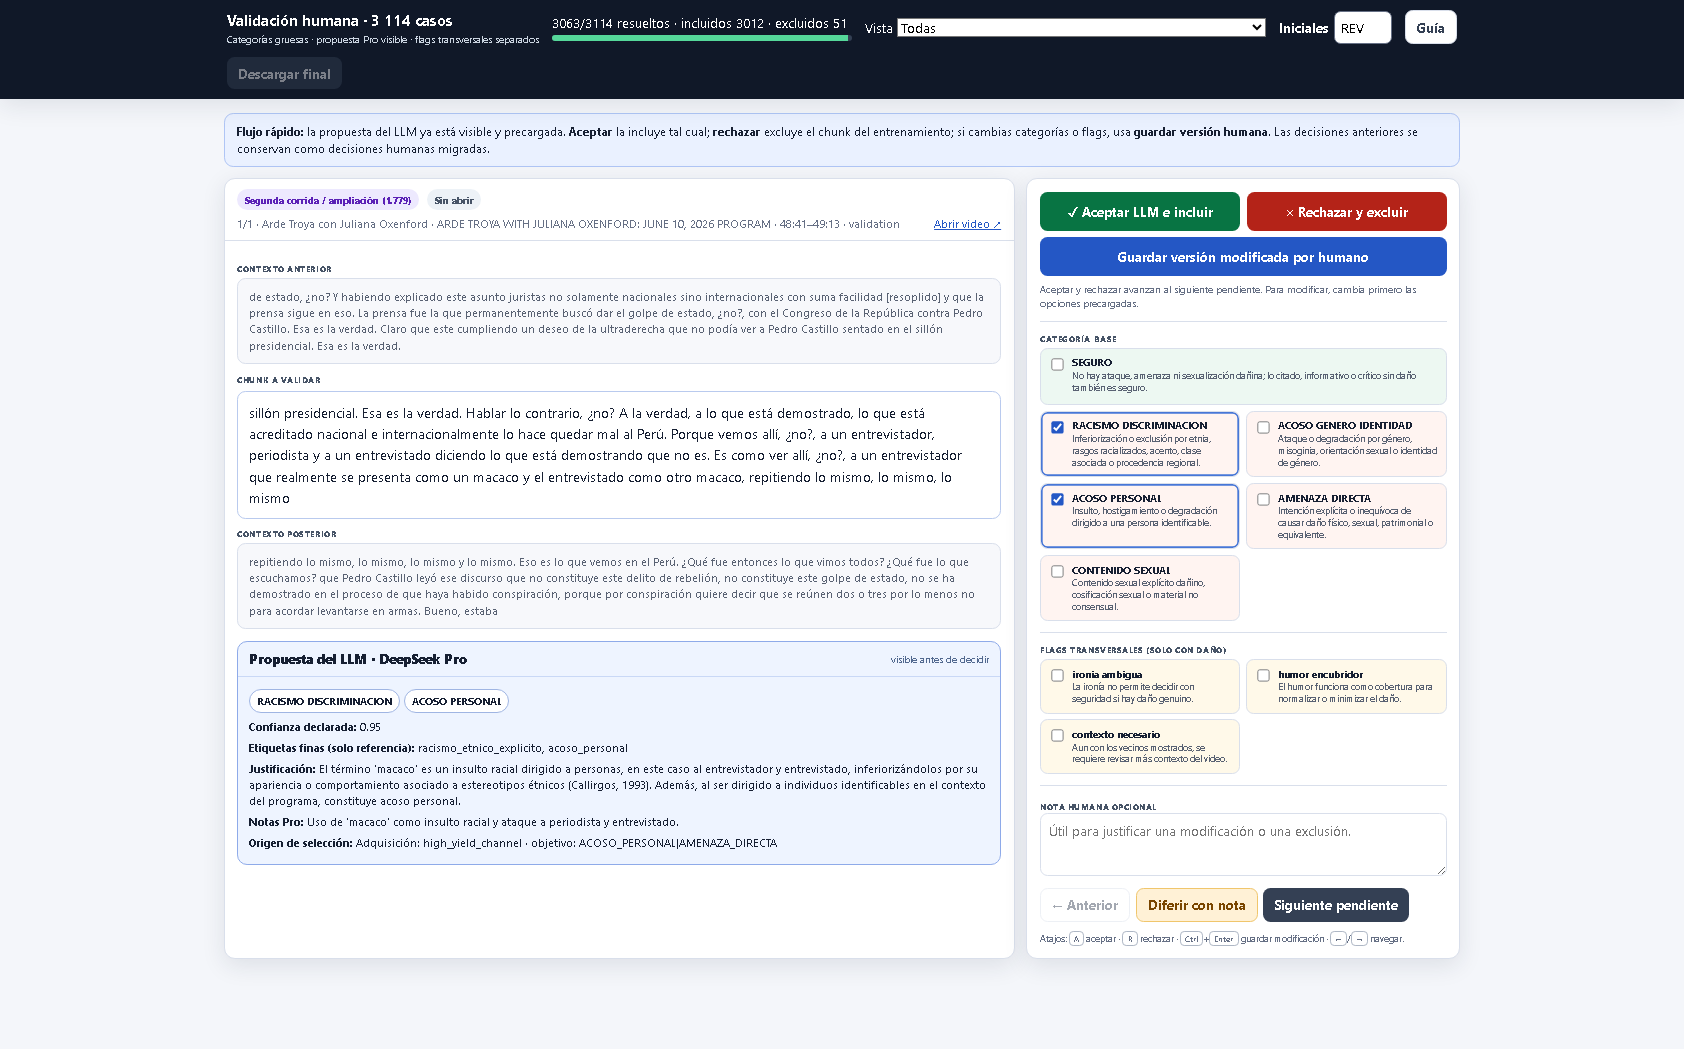
\includegraphics[width=\linewidth,height=52mm,keepaspectratio]{assets/captura_entorno_etiquetado.png}
    \end{column}
    \begin{column}{.29\textwidth}
      \smallcard{Blue}{Contexto visible}{Video, texto y tramo temporal se revisan juntos.}
      \vspace{2mm}
      \smallcard{Purple}{Decisión estructurada}{Categorías explícitas y observaciones reducen ambigüedad operativa.}
      \vspace{2mm}
      \smallcard{Teal}{Trazabilidad}{La acción queda vinculada a usuario, instante y versión.}
    \end{column}
  \end{columns}
  \takeaway{El frontend implementa la taxonomía mediante una decisión estructurada, repetible y auditable.}
  \resultNote{Captura histórica del frontend; la paridad funcional del frontend activo v2.1 está documentada en \texttt{docs/PARIDAD\_FRONTENDS\_ACTIVOS.md}.}
\end{frame}

\section{4. Entrenamiento y ensembles}

\chapterdivider{04}{Entrenamiento y ensembles}
  {Comparación de familias, adaptación de Qwen y estrategias de combinación de modelos.}
  {MODELOS CLÁSICOS \quad TRANSFORMERS \quad QWEN \quad ENSEMBLES}{Purple}

\begin{frame}[shrink=2]{Familias de modelos evaluadas}
  \framesubtitle{Una cartera diversa equilibra costo, contexto y desempeño}
  \begin{columns}[T,onlytextwidth]
    \begin{column}{.48\textwidth}
      \smallcard{Blue}{Modelos clásicos}{Frecuencia de término--frecuencia inversa de documento (TF--IDF) y clasificadores lineales: rápidos, interpretables y competitivos con señales léxicas fuertes~\cite{sparckjones1972idf,cox1958logistic,cortes1995svm}.}
      \vspace{2mm}
      \smallcard{Purple}{Transformers}{MiniLM/E5 y cascadas: representaciones contextuales con distinta relación entre costo y capacidad~\cite{vaswani2017attention,wang2020minilm,wang2022e5,wang2024e5}.}
    \end{column}
    \begin{column}{.48\textwidth}
      \smallcard{Gold}{Qwen + LoRA}{Adaptación de bajo rango (LoRA) de un modelo Qwen para capturar lenguaje y categorías con más contexto, actualizando una fracción de parámetros~\cite{qwen2025qwen3,hu2022lora}.}
      \vspace{2mm}
      \smallcard{Teal}{Ensembles}{Combinan probabilidades o decisiones de miembros diversos para reducir errores no coincidentes~\cite{dietterich2000ensemble,lam1997majority}.}
    \end{column}
  \end{columns}
  \vspace{3mm}
  \begin{center}
    \pill{Blue}{28 candidatos individuales}\quad
    \pill{Teal}{5 reglas + 2 optimizadas}\quad
    \pill{Purple}{validación anidada por vídeo}
  \end{center}
  \takeaway{La comparación conjunta aprovecha la complementariedad entre señales léxicas, representaciones contextuales y Qwen adaptado.}
  \resultNote{Inventario verificable de \texttt{comparacion\_individual\_ensemble\_validation.json}; arquitectura: \texttt{docs/ARQUITECTURAS\_MODELOS\_03.md}.}
\end{frame}

\begin{frame}{Diseño del entrenamiento y evaluación}
  \framesubtitle{Selección sin fuga y test abierto una sola vez}
  \centering
  \begin{tikzpicture}[
    n/.style={draw,rounded corners=3pt,text width=27mm,minimum height=22mm,align=center,inner sep=2mm,font=\scriptsize},
    a/.style={-{Stealth[length=2mm]},thick,draw=Muted},
    lab/.style={font=\tiny,text=Muted,align=center}]
    \node[n,draw=Blue!50,fill=Blue!7] (tr) {\textbf{TRAIN}\par ajuste de pesos\par 123\,239 chunks};
    \node[n,draw=Purple!50,fill=Purple!7,right=5mm of tr] (oof) {\textbf{Fuera de muestra (OOF)}\par 5 pliegues por video};
    \node[n,draw=Gold!55,fill=Gold!9,right=5mm of oof] (va) {\textbf{VALIDATION}\par comparación, bootstrap y congelación};
    \node[n,draw=Teal!50,fill=Teal!7,right=5mm of va] (te) {\textbf{TEST}\par apertura única\par 22\,684 chunks};
    \draw[a] (tr)-- node[lab,above]{aprende} (oof);
    \draw[a] (oof)-- node[lab,above]{estima sin fuga} (va);
    \draw[a] (va)-- node[lab,above]{congela antes de abrir} (te);
  \end{tikzpicture}
  \vspace{5mm}
  \begin{columns}[T,onlytextwidth]
    \begin{column}{.31\textwidth}
      \smallcard{Blue}{Unidad de grupo}{Un video completo pertenece a un solo split o fold.}
    \end{column}
    \begin{column}{.31\textwidth}
      \smallcard{Gold}{Métricas adecuadas}{Área bajo la curva precisión--sensibilidad (AUPRC) para daños raros; BA para la compuerta desbalanceada~\cite{saito2015pr,davis2006pr,brodersen2010balanced}.}
    \end{column}
    \begin{column}{.31\textwidth}
      \smallcard{Teal}{Evidencia temporal}{La selección queda firmada antes de consultar test.}
    \end{column}
  \end{columns}
  \takeaway{El test no decide el ganador: estima una vez el desempeño de la política ya congelada.}
\end{frame}

\begin{frame}[shrink=5]{Qwen y MiniLM: escala, ajuste y precisión numérica}
  \framesubtitle{LoRA reduce los parámetros ajustados; BF16 no equivale a cuantización}
  \begin{columns}[T,onlytextwidth]
    \begin{column}{.49\textwidth}
      \smallcard{Purple}{Qwen3-0.6B-Base}{596,05 millones de parámetros de base; 28 capas, dimensión 1\,024 y atención agrupada 16Q/8KV. Contexto nativo 32\,768; entrada operativa 256 tokens~\cite{qwen2025qwen3,hf2026qwen06bcard}.}
      \vspace{1.5mm}
      \smallcard{Gold}{Adaptación LoRA}{Rango 8, $\alpha=16$, \emph{dropout} 0,05 y matrices Q/K/V/O. Se ajustan 2\,316\,288 parámetros (0,39\%); adaptador FP32 de 9,29 MB~\cite{hu2022lora}.}
      \vspace{1.5mm}
      \metriccard{Purple}{0,831}{BA binaria OOF}{mejor individuo del ranking}
    \end{column}
    \begin{column}{.49\textwidth}
      \smallcard{Blue}{MiniLM-L12-v2}{117\,662\,230 parámetros con la cabeza local de 22 salidas; 12 capas, dimensión 384, 12 cabezas y entrada de 128 tokens~\cite{wang2020minilm,hf2026minilmcard}.}
      \vspace{1.5mm}
      \smallcard{Teal}{Ajuste completo}{El candidato de 03\_07 ajusta toda la red; solo el piloto de longitud congela el encoder. BA OOF 0,814 y macro-AUPRC 0,476.}
      \vspace{1.5mm}
      \smallcard{Coral}{Sin cuantización}{Ninguno usa 4/8 bits, NF4 ni QLoRA. BF16 es precisión mixta de cálculo en GPU; en CPU la carga estándar queda sin cuantizar.}
    \end{column}
  \end{columns}
  \takeaway{Qwen logra el mejor resultado individual ajustando menos de 0,4\% del clasificador; MiniLM ofrece una referencia compacta, aunque no integra el ensemble final.}
  \resultNote{Conteos verificados en los tensores y configuraciones locales. El miembro Transformer del ensemble es la cascada E5 v2, no MiniLM.}
\end{frame}

\begin{frame}[shrink=8]{Entrenamientos Qwen realizados}
  \framesubtitle{La longitud y la pérdida cambian; el backbone y el contrato permanecen fijos}
  \begin{columns}[T,onlytextwidth]
    \begin{column}{.49\textwidth}
      \smallcard{Purple}{03\_05 · LoRA base, 128 tokens}{BCE ponderada y 22 logits enmascarados; $10^{-4}$, lote efectivo 8 y hasta cuatro épocas. El ajuste paró tras la época 3 y restauró la época 2. \textbf{Ganador Qwen y mejor individuo}: BA 0,831; AUPRC 0,516.}
      \vspace{1.5mm}
      \smallcard{Blue}{03\_05 · LoRA continuado, 256}{Warm-start del anterior, optimizador nuevo y hasta cuatro épocas adicionales. Reduce truncamiento de 56,1\% a 0,002\%; AUPRC 0,523 y F1 0,572, pero BA 0,830.}
    \end{column}
    \begin{column}{.49\textwidth}
      \smallcard{Gold}{03\_06 · barrido LoRA estructurado}{Tres continuaciones de una época, $2\times10^{-5}$ y $\lambda=0/0,02/0,05$ para penalizar \texttt{SEGURO}+daño. Gana $\lambda=0,05$ dentro del barrido: BA 0,819; AUPRC 0,500.}
      \vspace{1.5mm}
      \smallcard{Coral}{03\_06 · ajuste completo histórico}{Única ruta \textbf{sin LoRA}: cuatro épocas y $\lambda=0,2$. Fue más costosa y rindió peor: AUPRC 0,243; falso seguro 0,775. Se conserva como antecedente descartado.}
    \end{column}
  \end{columns}
  \takeaway{El mejor Qwen no fue el más largo: el LoRA base maximiza BA; el contexto 256 mejora categorías específicas y los estructurados no compensan la pérdida global.}
  \resultNote{Los dos identificadores de contexto 256 del ranking reproducen las mismas métricas; no constituyen réplicas independientes. El ensemble usa el LoRA base.}
\end{frame}

\begin{frame}[shrink=12]{Metodología del ensemble optimizado}
  \framesubtitle{Calibración por miembro y pesos aprendidos sin consultar test}
  \centering
  \begin{tikzpicture}[
    n/.style={draw,rounded corners=4pt,text width=30mm,minimum height=16mm,align=center,inner sep=1.5mm,font=\scriptsize},
    a/.style={-{Stealth[length=2mm]},very thick,draw=Muted}]
    \node[n,draw=Blue!50,fill=Blue!7] (cl) {\textbf{Clásico}\par regresión logística, $C=0,5$};
    \node[n,draw=Purple!50,fill=Purple!7,right=5mm of cl] (tr) {\textbf{Transformer}\par cascade v2};
    \node[n,draw=Gold!55,fill=Gold!9,right=5mm of tr] (qw) {\textbf{Qwen}\par Qwen + LoRA};
    \node[n,draw=Teal!60,fill=Teal!9,below=7mm of tr,text width=43mm,minimum height=18mm] (mean) {\textbf{Mezcla convexa}\quad $E_c=0{,}10p_{C,c}+0{,}65p_{T,c}+0{,}25p_{Q,c}$};
    \node[n,draw=Navy!60,fill=Navy!7,right=12mm of mean,text width=36mm,minimum height=18mm] (out) {\textbf{Política}\par 5 salidas + \texttt{NEEDS\_REVIEW}};
    \draw[a] (cl.south)--(mean.north); \draw[a] (tr.south)--(mean.north); \draw[a] (qw.south)--(mean.north); \draw[a] (mean)--(out);
  \end{tikzpicture}
  \vspace{2mm}
  \begin{columns}[T,onlytextwidth]
    \begin{column}{.47\textwidth}
      \smallcard{Teal}{1 · Ajuste interno}{En cada train externo, 5 pliegues por vídeo generan scores OOF; allí se ajustan Platt y umbrales, y se evalúan 861 ternas no negativas de paso 0,025.}
    \end{column}
    \begin{column}{.47\textwidth}
      \smallcard{Purple}{2 · Estimación externa}{Se elige por BA $\uparrow$, $R_{0,67}\downarrow$ y macro-AUPRC $\uparrow$; los pesos se aplican al quinto externo intacto. Los 5 quintos forman el ranking anidado.}
    \end{column}
  \end{columns}
  \takeaway{Se optimizan todas las mezclas parametrizadas; unión e intersección no reciben coeficientes artificiales.}
  \externalNote{Calibración~\cite{platt1999probabilistic}; selección anidada~\cite{cawley2010selection}; combinación aprendida~\cite{wolpert1992stacked,vanderlaan2007superlearner}. Malla y objetivo lexicográfico: propuesta propia.}
\end{frame}

\begin{frame}[shrink=9]{Estrategias de ensemble evaluadas}
  \framesubtitle{Cinco reglas base y dos variantes optimizadas bajo el mismo protocolo}
  \begin{columns}[T,onlytextwidth]
    \begin{column}{.31\textwidth}
      \smallcard{Blue}{Clásico}{Regresión logística con $C=0,5$.}
    \end{column}
    \begin{column}{.31\textwidth}
      \smallcard{Purple}{Transformer}{Arquitectura cascade v2.}
    \end{column}
    \begin{column}{.31\textwidth}
      \smallcard{Gold}{Qwen}{Qwen adaptado mediante LoRA.}
    \end{column}
  \end{columns}
  \vspace{2.5mm}
  \centering\scriptsize
  \begin{tabularx}{\textwidth}{@{}p{26mm}Xrrrr@{}}
    \toprule
    \textbf{Regla} & \textbf{Operación / pesos C--T--Q} & \textbf{BA} & $\boldsymbol{R_{.67}}$ & \textbf{AP} & \textbf{F1}\\
    \midrule
    \rowcolor{Teal!12}\textbf{Suave optimizado} & 0,100 / 0,650 / 0,250. & \textbf{0,8366} & \textbf{0,1587} & 0,5506 & 0,5618\\
    Ponderado AUPRC & 0,332 / 0,311 / 0,357. & 0,8360 & 0,1612 & \textbf{0,5614} & 0,5675\\
    Unión & Máximo; sin coeficientes. & 0,8334 & 0,1684 & 0,5369 & 0,5621\\
    Promedio simple & 1/3 / 1/3 / 1/3. & 0,8328 & 0,1673 & 0,5604 & \textbf{0,5703}\\
    Duro optimizado & 0,300 / 0,325 / 0,375 sobre votos. & 0,8272 & 0,1731 & 0,4547 & 0,5584\\
    Mayoría dura & 1/3 / 1/3 / 1/3 sobre votos. & 0,8272 & 0,1731 & 0,4415 & 0,5638\\
    Intersección & Mínimo; sin coeficientes. & 0,8149 & 0,1887 & 0,5131 & 0,5373\\
    \bottomrule
  \end{tabularx}
  \vspace{2mm}
  \takeaway{La optimización cambia el ganador: se congela únicamente la mezcla suave 0,10/0,65/0,25.}
  \resultNote{03\_07b, validación OOF externa anidada; cuaderno local ejecutado y hashes de entrada verificados.}
\end{frame}

\begin{frame}[shrink=4]{Métricas de ranking: qué miden}
  \framesubtitle{BA es la métrica principal; macro-AUPRC protege los daños y F1 describe umbrales}
  \scriptsize
  \renewcommand{\arraystretch}{1.18}
  \begin{tabularx}{\textwidth}{@{}>{\bfseries\color{Navy}}p{30mm}p{36mm}X>{\centering\arraybackslash}p{15mm}@{}}
    \toprule
    Métrica & Definición operativa & Qué significa & Mejor \\
    \midrule
    Exactitud balanceada (BA) & $\tfrac{1}{2}(\text{sensibilidad}+\text{especificidad})$ en ANY\_DAMAGE & Promedia la capacidad de detectar daño y reconocer contenido seguro sin dejar que la clase mayoritaria domine. & $\uparrow$ \\
    \rowcolor{Blue!5}
    Macro-AUPRC de daño & Media no ponderada de las cuatro áreas bajo la curva precisión--sensibilidad & Evalúa el ordenamiento de positivos a través de todos los umbrales y da igual peso a cada daño raro. & $\uparrow$ \\
    Macro-F1 de daño & Media del F1 por daño; $F1=2PR/(P+R)$ & Resume precisión y sensibilidad después de fijar umbrales; no incorpora verdaderos negativos. & $\uparrow$ \\
    \rowcolor{Blue!5}
    $R_{0,67}$ & $0,67\,\text{FNR}+0,33\,\text{FPR}$ & FNR: daño omitido; FPR: falsa alerta. Penaliza la omisión $0,67/0,33\simeq2,03$ veces y se minimiza. & $\downarrow$ \\
    Carga de revisión & Fracción enviada a \texttt{NEEDS\_REVIEW} & Capacidad humana necesaria; siempre se interpreta junto con BA/riesgo de la ruta automática. & $\downarrow$ \\
    \bottomrule
  \end{tabularx}
  \vspace{2mm}
  \takeaway{La métrica principal es BA de ANY\_DAMAGE OOF a cobertura completa. Además, $R_{0,50}=1-\mathrm{BA}$; usar 0,67 desplaza el desempate hacia evitar daño omitido.}
  \externalNote{BA ante desbalance~\cite{brodersen2010balanced}; precisión--sensibilidad~\cite{saito2015pr,davis2006pr}; criterio local completo en \texttt{docs/CRITERIO\_SELECCION\_MODELOS\_03.md}.}
\end{frame}

\begin{frame}[shrink=5]{Cómo leer el ranking y por qué no usar otras métricas}
  \framesubtitle{La interpretación evita convertir porcentajes distintos en una sola “nota”}
  \begin{columns}[T,onlytextwidth]
    \begin{column}{.48\textwidth}
      \smallcard{Teal}{BA 0,8366}{No significa “83,66\,\% de chunks correctos”: es el promedio de sensibilidad y especificidad de la compuerta binaria, estimado en pliegues externos.}
      \vspace{1.5mm}
      \smallcard{Gold}{Macro-AUPRC 0,5506}{No significa “55,06\,\% de aciertos”: es el área precisión--sensibilidad media de los cuatro daños; solo se compara sobre el mismo panel y prevalencia.}
      \vspace{1.5mm}
      \smallcard{Purple}{Macro-F1 0,5618}{Describe las decisiones por categoría en umbrales aprendidos dentro de cada pliegue; una categoría rara pesa lo mismo que una frecuente.}
    \end{column}
    \begin{column}{.48\textwidth}
      \smallcard{Coral}{No accuracy ni micro-F1}{La abundancia de SEGURO puede producir una cifra alta aun cuando se omita daño; micro/weighted privilegia las etiquetas con mayor soporte.}
      \vspace{1.5mm}
      \smallcard{Blue}{No ROC-AUC como criterio principal}{Con positivos raros, precisión--sensibilidad muestra mejor cuántas alertas relevantes aparecen entre las predicciones positivas~\cite{saito2015pr,davis2006pr}.}
      \vspace{1.5mm}
      \smallcard{Green}{No suma de indicadores}{BA ya contiene FNR y FPR; sumarlos contaría dos veces errores correlacionados. Calibración y carga humana tienen escalas y utilidades distintas.}
    \end{column}
  \end{columns}
  \takeaway{El ranking es lexicográfico con salvaguardas: primero equilibrio DAÑO--SEGURO, luego desempeño multietiqueta, frontera de Pareto y costos como desempate.}
\end{frame}

\begin{frame}[shrink=7]{Criterio de selección y análisis estadístico}
  \framesubtitle{Desempeño, salvaguardas e incertidumbre en un solo protocolo}
  \begin{columns}[T,onlytextwidth]
    \begin{column}{.58\textwidth}
      \begin{enumerate}\setlength\itemsep{1.2mm}
        \item \textbf{Criterio primario:} mayor exactitud balanceada de ANY\_DAMAGE con predicciones OOF y cobertura completa.
        \item \textbf{Salvaguarda:} macro-AUPRC de los cuatro daños dentro de un margen de no inferioridad predeclarado.
        \item \textbf{Frontera de Pareto:} descarta opciones dominadas en sensibilidad/especificidad y desempeño por categoría.
        \item \textbf{Desempate:} menor riesgo $R_{0,67}$ y luego mayor macro-AUPRC.
        \item \textbf{Incertidumbre:} 2\,000 réplicas pareadas por video; se reportan IC y $p$ sin inflar la evidencia.
      \end{enumerate}
    \end{column}
    \begin{column}{.38\textwidth}
      \smallcard{Blue}{1 · BA decide}{Suave optimizado 0,8366; ponderado 0,8360; promedio simple 0,8328.}
      \vspace{2mm}
      \smallcard{Gold}{2 · Salvaguarda}{AUPRC 0,5506; el ponderado alcanza 0,5614, pero no desplaza al líder del criterio primario.}
      \vspace{2mm}
      \smallcard{Purple}{3 · Riesgo y pesos}{$R_{0,67}=0,1587$; ajuste final C/T/Q = 0,10/0,65/0,25.}
    \end{column}
  \end{columns}
  \takeaway{El suave optimizado es el único seleccionado; frente al ponderado, $\Delta\mathrm{BA}=+0{,}00059$, IC95\,\% $[-0,00367;0,00509]$, $p=0,804$: ventaja inconclusa.}
  \externalNote{Bootstrap pareado por video~\cite{field2007clusterbootstrap}; criterio interno: \texttt{docs/CRITERIO\_SELECCION\_MODELOS\_03.md}.}
\end{frame}

\section{5. Resultados finales}

\chapterdivider{05}{Resultados finales}
  {Ganadores globales, por tipo y por categoría; test natural y revisión humana.}
  {VALIDACIÓN \quad TEST NATURAL \quad CATEGORÍAS \quad REVISIÓN}{Gold}

\begin{frame}[shrink=5]{Ranking global en validación}
  \framesubtitle{La combinación multifamilia obtiene el mejor resultado global}
  \begin{columns}[T,onlytextwidth]
    \begin{column}{.72\textwidth}
      \centering
      \begin{tikzpicture}
        \begin{axis}[
          xbar,width=.92\linewidth,height=56mm,xmin=.81,xmax=.839,
          symbolic y coords={Intersección,Mayoría,Duro optimizado,Promedio,Unión,Ponderado,Suave optimizado},
          ytick=data,axis y line*=left,axis x line*=bottom,
          xtick={.81,.82,.83,.84},scaled x ticks=false,
          tick label style={font=\tiny},nodes near coords,point meta=x,
          every node near coord/.append style={font=\tiny\bfseries,/pgf/number format/fixed,/pgf/number format/precision=4},
          enlarge y limits=.08]
          \addplot[fill=Blue!45,draw=Blue] coordinates {(.8149,Intersección) (.8272,Mayoría) (.8272,Duro optimizado) (.8328,Promedio) (.8334,Unión) (.8360,Ponderado)};
          \addplot[fill=Teal!80,draw=Teal] coordinates {(.8366,Suave optimizado)};
        \end{axis}
      \end{tikzpicture}
      {\tiny Exactitud balanceada anidada de las siete variantes de ensemble.}
    \end{column}
    \begin{column}{.25\textwidth}
      \metriccard{Teal}{0,8366}{BA anidada}{ANY\_DAMAGE; cobertura completa}
      \vspace{2mm}
      \metriccard{Purple}{0,5506}{macro-AUPRC OOF}{cuatro daños}
      \vspace{2mm}
      \metriccard{Blue}{0,5618}{macro-F1}{cuatro daños}
    \end{column}
  \end{columns}
  \takeaway{El mejor punto global integra clásico + Transformer + Qwen; el resultado respalda la diversidad de la cartera, no una arquitectura única.}
  \resultNote{03\_07b, \texttt{optimizacion\_ensembles\_validation.json}; único ganador actual: \texttt{ensemble\_soft\_optimized}.}
\end{frame}

\begin{frame}[shrink=6]{Mejor modelo por tipo}
  \framesubtitle{La mejora se mantiene desde los modelos clásicos hasta el ensemble}
  \begin{columns}[T,onlytextwidth]
    \begin{column}{.53\textwidth}
      \centering
      \begin{tikzpicture}
        \begin{axis}[
          xbar,width=.97\linewidth,height=52mm,
          xmin=.76,xmax=.85,
          symbolic y coords={Clásico,Transformer,Qwen,Ensemble},ytick=data,
          axis y line*=left,ytick style={draw=none},axis x line*=bottom,
          scaled x ticks=false,
          xtick={.76,.78,.80,.82,.84},
          tick label style={font=\scriptsize},
          nodes near coords,nodes near coords align={horizontal},
          every node near coord/.append style={font=\scriptsize\bfseries,color=Ink},
          enlarge y limits=.18]
          \addplot[fill=Blue!70,draw=Blue] coordinates {(.801415,Clásico) (.816981,Transformer) (.831368,Qwen) (.836557,Ensemble)};
        \end{axis}
      \end{tikzpicture}
      {\tiny Exactitud balanceada binaria OOF, validación. Eje truncado para mostrar diferencias.}
    \end{column}
    \begin{column}{.44\textwidth}
      \scriptsize
      \begin{tabularx}{\linewidth}{@{}Xrr@{}}
        \toprule
        \textbf{Ganador de tipo} & \textbf{macro-AUPRC} & \textbf{F1 macro}\\
        \midrule
        Regresión logística & 0,479 & 0,503\\
        Cascade v2 & 0,449 & 0,519\\
        Qwen + LoRA & 0,516 & 0,553\\
        \rowcolor{Teal!10}\textbf{Suave optimizado} & \textbf{0,551} & \textbf{0,562}\\
        \bottomrule
      \end{tabularx}
      \vspace{3mm}
      \smallcard{Teal}{Ganancia acumulada}{El ensemble supera al mejor clásico en +3,51 puntos de BA y +7,16 puntos de macro-AUPRC.}
      \vspace{2mm}
      \smallcard{Purple}{Lectura honesta}{Las diferencias entre familias no prueban causalidad arquitectónica: resumen los mejores candidatos ejecutados.}
    \end{column}
  \end{columns}
  \resultNote{03\_07a, \texttt{mejores\_por\_tipo\_validation.csv}; cifras sin redondear conservadas en el archivo fuente.}
\end{frame}

\begin{frame}[shrink=8]{Frontera de Pareto e incertidumbre estadística}
  \framesubtitle{Selección reproducible con una diferencia estadística no concluyente}
  \begin{columns}[T,onlytextwidth]
    \begin{column}{.50\textwidth}
      \centering
      \begin{tikzpicture}
        \begin{axis}[
          width=\linewidth,height=55mm,xmin=.43,xmax=.57,ymin=.81,ymax=.84,
          xlabel={macro-AUPRC},ylabel={BA},
          tick label style={font=\tiny},label style={font=\scriptsize},
          grid=both,grid style={Line!12}]
          \addplot[only marks,mark=*,mark size=2.2pt,Muted] coordinates {(.5369,.8334) (.5604,.8328) (.4547,.8272) (.4415,.8272) (.5131,.8149)};
          \addplot[only marks,mark=diamond*,mark size=3pt,Gold] coordinates {(.5614,.8360)};
          \addplot[only marks,mark=star,mark size=4pt,Teal] coordinates {(.5506,.8366)};
          \node[font=\tiny\bfseries,text=Teal,anchor=south east] at (axis cs:.5506,.8366) {suave opt.};
          \node[font=\tiny\bfseries,text=Gold,anchor=north west] at (axis cs:.5614,.8360) {ponderado};
        \end{axis}
      \end{tikzpicture}
    \end{column}
    \begin{column}{.47\textwidth}
      \smallcard{Teal}{Selección vigente}{\texttt{ensemble\_soft\_optimized} ocupa el rango uno y es el único ganador actual.}
      \vspace{2mm}
      \smallcard{Gold}{Rival más cercano}{El ponderado por AUPRC queda a $-0,00059$ de BA.}
      \vspace{2mm}
      \smallcard{Purple}{Incertidumbre}{IC95\,\% pareado para ganador menos rival: $[-0,00367;\ 0,00509]$; $p=0,804$. Pesos suaves variables entre pliegues.}
    \end{column}
  \end{columns}
  \takeaway{Hay un único seleccionado por la regla; su ventaja estadística permanece inconclusa y se reporta como limitación.}
  \externalNote{Bootstrap agrupado~\cite{field2007clusterbootstrap}; pruebas pareadas y ajuste múltiple~\cite{dror2018significance,holm1979multiple}.}
\end{frame}

\begin{frame}[shrink=5]{Resultados en test de prevalencia natural}
  \framesubtitle{Alta sensibilidad sobre 22\,684 chunks en condiciones naturales}
  \begin{columns}[T,onlytextwidth]
    \begin{column}{.31\textwidth}
      \metriccard{Teal}{0,846}{exactitud balanceada}{cobertura completa}
    \end{column}
    \begin{column}{.31\textwidth}
      \metriccard{Coral}{0,894}{sensibilidad al daño}{omite 10,60\,\% del daño}
    \end{column}
    \begin{column}{.31\textwidth}
      \metriccard{Blue}{0,531}{AP de daño}{prevalencia natural 7,94\,\%}
    \end{column}
  \end{columns}
  \vspace{4mm}
  \begin{columns}[T,onlytextwidth]
    \begin{column}{.50\textwidth}
      \centering\scriptsize
      \begin{tabular}{lrr}
        \toprule
         & \textbf{Pred. daño} & \textbf{Pred. seguro}\\
        \midrule
        \textbf{Daño real} & \cellcolor{Teal!15}1\,611 & \cellcolor{Coral!12}191\\
        \textbf{Seguro real} & \cellcolor{Gold!13}4\,221 & \cellcolor{Blue!12}16\,661\\
        \bottomrule
      \end{tabular}
      \par\vspace{1mm}{\tiny Matriz de confusión de la compuerta ANY\_DAMAGE.}
    \end{column}
    \begin{column}{.46\textwidth}
      \smallcard{Gold}{Compromiso actualizado}{La especificidad sube a 0,798 frente al promedio simple, mientras la sensibilidad baja; BA cambia solo +0,00004.}
      \vspace{2mm}
      \smallcard{Purple}{Desempeño por daños}{Macro-AUPRC = 0,412; macro-F1 = 0,423 sobre cuatro categorías.}
    \end{column}
  \end{columns}
  \takeaway{A prevalencia natural, el sistema encuentra 1\,611 de 1\,802 chunks dañinos; el test evalúa la fórmula, no vuelve a escogerla.}
  \resultNote{03\_07, \texttt{test\_final\_abierto\_una\_vez.json}; 22\,684 chunks de 674 videos.}
\end{frame}

\begin{frame}[shrink=5]{Política de revisión humana}
  \framesubtitle{Los casos inciertos se reservan para supervisión humana}
  \begin{columns}[T,onlytextwidth]
    \begin{column}{.60\textwidth}
      \centering
      \begin{tikzpicture}
        \begin{axis}[
          ybar,width=\linewidth,height=55mm,ymin=0,ymax=1,
          symbolic x coords={BA,Sensibilidad,Especificidad,F1},xtick=data,
          ylabel={proporción},
          tick label style={font=\scriptsize},
          legend style={font=\tiny,at={(.5,1.02)},anchor=south,legend columns=2,draw=none},
          nodes near coords,point meta=y,
          every node near coord/.append style={font=\tiny,/pgf/number format/fixed,/pgf/number format/precision=3}]
          \addplot[fill=Blue!55,draw=Blue] coordinates {(BA,.845935) (Sensibilidad,.894007) (Especificidad,.797864) (F1,.422059)};
          \addplot[fill=Teal!65,draw=Teal] coordinates {(BA,.924894) (Sensibilidad,.902240) (Especificidad,.947548) (F1,.660701)};
          \legend{Cobertura completa,Ruta automática}
        \end{axis}
      \end{tikzpicture}
    \end{column}
    \begin{column}{.37\textwidth}
      \metriccard{Green}{72,7\,\%}{cobertura automática}{16\,500 chunks resueltos sin derivación}
      \vspace{2mm}
      \metriccard{Gold}{27,3\,\%}{carga de revisión}{6\,184 chunks derivados}
      \vspace{2mm}
      \smallcard{Purple}{Política congelada}{$\delta=0,03$; revisa cercanía a umbrales e incoherencias entre compuerta y categorías.}
    \end{column}
  \end{columns}
  \takeaway{0,925 de BA aplica al 72,7\,\% automático; el 27,3\,\% restante es la salvaguarda humana.}
  \externalNote{Clasificación selectiva y aprendizaje con derivación~\cite{geifman2017selective,mozannar2020defer}; calibración~\cite{guo2017calibration}.}
\end{frame}

\begin{frame}[shrink=5]{Resultados por categoría en test natural}
  \framesubtitle{Contenido sexual y acoso presentan los mejores resultados}
  \begin{columns}[T,onlytextwidth]
    \begin{column}{.66\textwidth}
      \centering
      \begin{tikzpicture}
        \begin{axis}[
          xbar,width=.985\linewidth,height=53mm,xmin=0,xmax=.7,
          symbolic y coords={Género,Racismo,Acoso,Sexual},ytick=data,
          axis y line*=left,ytick style={draw=none},axis x line*=bottom,
          scaled x ticks=false,
          xtick={0,.1,.2,.3,.4,.5,.6,.7},
          tick label style={font=\scriptsize},
          legend style={font=\tiny,at={(.5,1.02)},anchor=south,legend columns=2,draw=none},
          nodes near coords,point meta=x,
          every node near coord/.append style={font=\tiny,/pgf/number format/fixed,/pgf/number format/precision=3},
          enlarge y limits=.14]
          \addplot[fill=Purple!58,draw=Purple] coordinates {(.268188,Género) (.358377,Racismo) (.445964,Acoso) (.575239,Sexual)};
          \addplot[fill=Teal!63,draw=Teal] coordinates {(.310484,Género) (.358608,Racismo) (.453441,Acoso) (.571429,Sexual)};
          \legend{AUPRC,F1}
        \end{axis}
      \end{tikzpicture}
    \end{column}
    \begin{column}{.30\textwidth}
      \smallcard{Teal}{Mayor desempeño}{CONTENIDO SEXUAL: AUPRC 0,575 y F1 0,571.}
      \vspace{2mm}
      \smallcard{Blue}{Zona intermedia}{ACOSO/AMENAZA: AUPRC 0,446 y F1 0,453.}
      \vspace{2mm}
      \smallcard{Coral}{Prioridad de mejora}{GÉNERO/IDENTIDAD: AUPRC 0,268 y F1 0,310.}
    \end{column}
  \end{columns}
  \takeaway{El promedio no basta: género/identidad y racismo requieren más ejemplos fronterizos, auditoría localizada y análisis de deriva.}
  \resultNote{Test natural; métricas de la predicción congelada por categoría, \texttt{metricas\_por\_categoria\_test.csv}.}
\end{frame}

\begin{frame}[shrink=5]{Mejor modelo por categoría en validación}
  \framesubtitle{Qwen y los ensembles se especializan en daños distintos}
  \begin{columns}[T,onlytextwidth]
    \begin{column}{.61\textwidth}
      \centering
      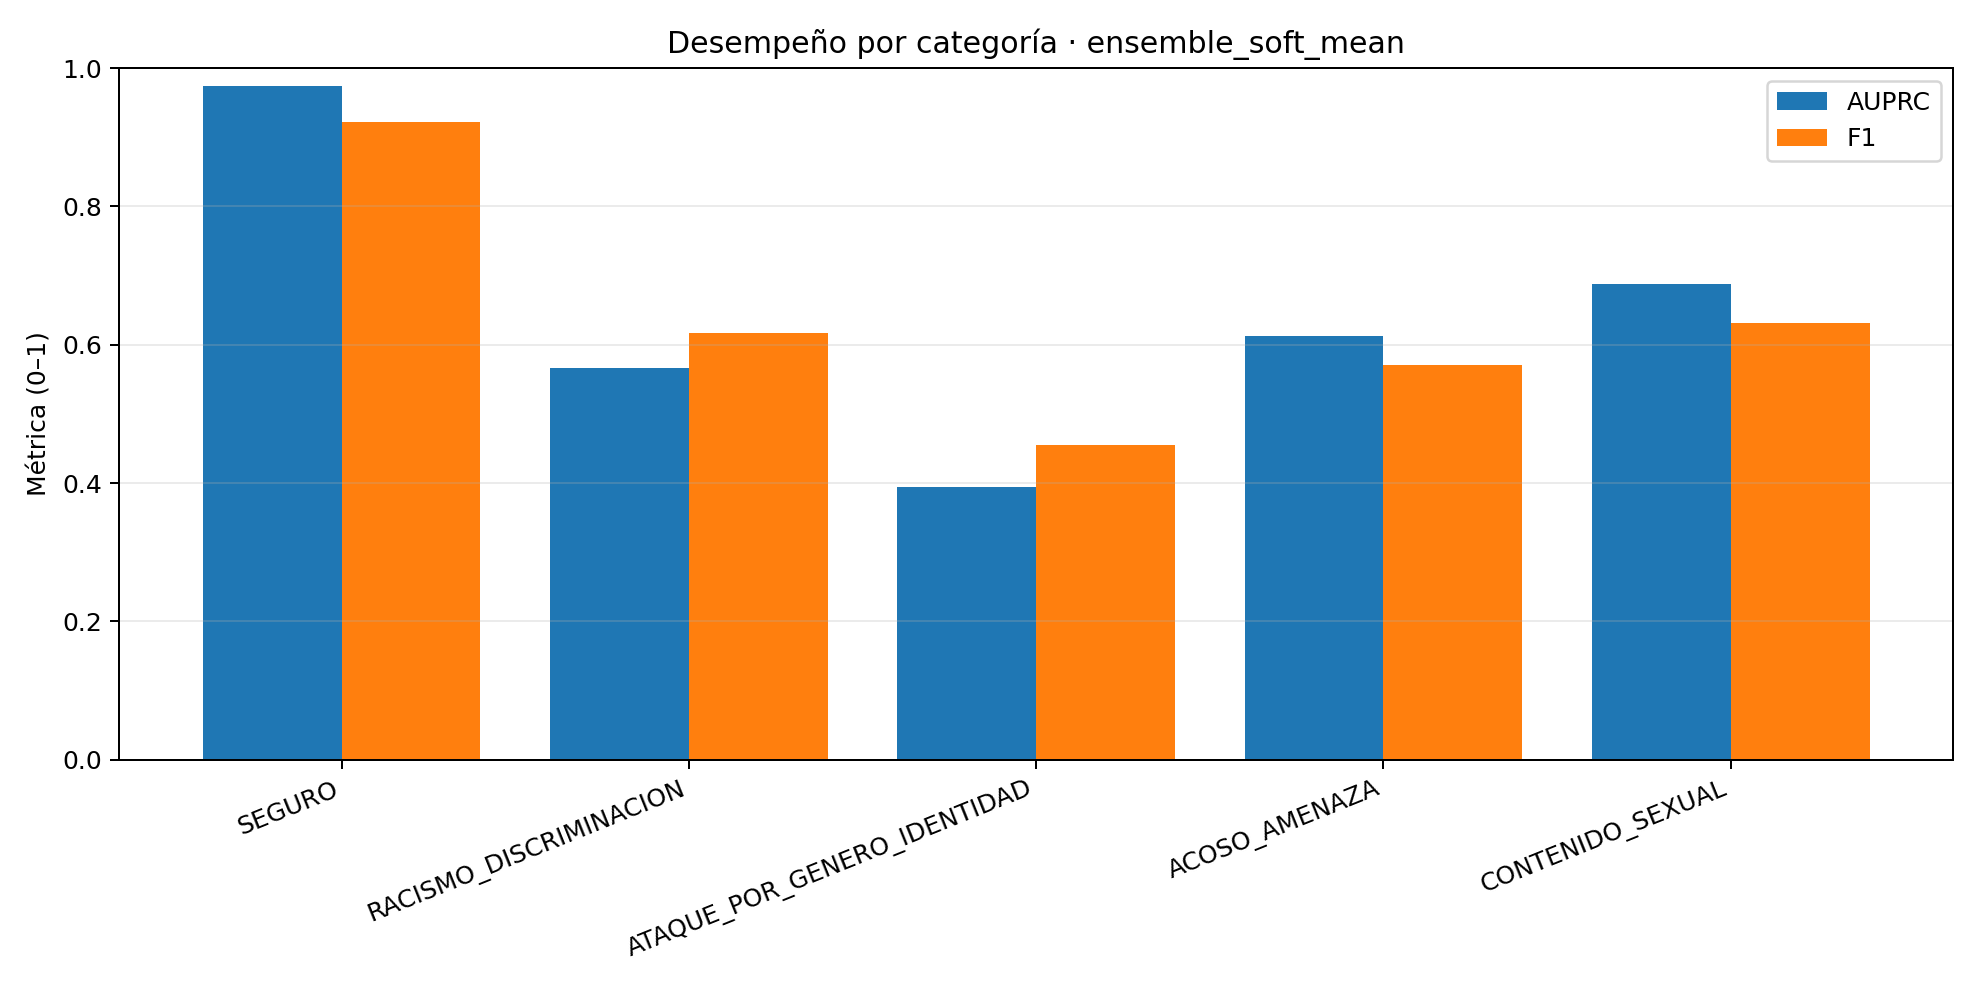
\includegraphics[width=\linewidth,height=52mm,keepaspectratio]{assets/seleccion_por_categoria_validation.png}
    \end{column}
    \begin{column}{.36\textwidth}
      \scriptsize
      \begin{tabularx}{\linewidth}{@{}>{\raggedright\arraybackslash}X>{\raggedright\arraybackslash}Xr@{}}
        \toprule
        \textbf{Categoría} & \textbf{Mejor AUPRC} & \textbf{Valor}\\
        \midrule
        Racismo & Qwen contexto 256 & 0,571\\
        Género & Qwen contexto 256 & 0,402\\
        Acoso & Ensemble ponderado & 0,614\\
        Sexual & Promedio simple (pantalla) & 0,688\\
        \bottomrule
      \end{tabularx}
      \vspace{3mm}
      \smallcard{Purple}{Ganadores por F1}{Qwen con contexto 256 gana racismo; voto mayoritario, género; ensemble por unión, acoso y sexual.}
      \vspace{2mm}
      \smallcard{Teal}{Decisión de producto}{Se congela un ganador global para operación reproducible y se conservan especialistas como evidencia para futuras rutas por categoría.}
    \end{column}
  \end{columns}
  \takeaway{La diversidad tiene valor observable: Qwen domina categorías semánticas difíciles y los ensembles lideran acoso/sexual.}
  \resultNote{Validación, \texttt{ganadores\_por\_categoria\_validation.csv}; estas selecciones descriptivas no reabren el test.}
\end{frame}

\section{6. Comparación externa}

\chapterdivider{06}{Comparación externa}
  {Contraste de resultados publicados y análisis crítico de comparabilidad.}
  {MÉTRICAS \quad CONTEXTO \quad RESULTADOS \quad BRECHAS}{Blue}

\begin{frame}[shrink=5]{Comparación contextual con el estado del arte}
  \framesubtitle{Resultados del mismo orden que trabajos publicados relacionados}
  \begin{columns}[T,onlytextwidth]
    \begin{column}{.66\textwidth}
      \centering
      \begin{tikzpicture}
        \begin{axis}[
          xbar,width=.96\linewidth,height=58mm,xmin=.55,xmax=.84,
          symbolic y coords={DETOXIS,Este trabajo,HateXplain,HatEval,OffendES,EXIST},
          ytick={DETOXIS,Este trabajo,HateXplain,HatEval,OffendES,EXIST},
          axis y line*=left,ytick style={draw=none},axis x line*=bottom,
          scaled x ticks=false,
          xtick={.55,.60,.65,.70,.75,.80},
          tick label style={font=\scriptsize},
          nodes near coords,point meta=x,
          every node near coord/.append style={font=\tiny\bfseries,/pgf/number format/fixed,/pgf/number format/precision=3},
          enlarge y limits=.12]
          \addplot[fill=Muted!45,draw=Muted] coordinates {(.6461,DETOXIS) (.687,HateXplain) (.730,HatEval) (.7839,OffendES) (.7944,EXIST)};
          \addplot[fill=Teal!75,draw=Teal] coordinates {(.662418,Este trabajo)};
        \end{axis}
      \end{tikzpicture}
      {\tiny F1 reportado; este trabajo usa vista test 4:1 y compuerta binaria congelada.}
    \end{column}
    \begin{column}{.31\textwidth}
      \smallcard{Teal}{Posición contextual}{F1 = 0,662: comparable con DETOXIS (0,646) y HateXplain (0,687).}
      \vspace{2mm}
      \smallcard{Gold}{No es una liga común}{HatEval 0,730; OffendES 0,784; EXIST 0,794, pero cambian corpus, idioma, prevalencia, etiquetas y partición.}
      \vspace{2mm}
      \smallcard{Purple}{Mayor amplitud local}{Aquí se integran cuatro daños peruanos, multietiqueta, marcas temporales y derivación humana.}
    \end{column}
  \end{columns}
  \takeaway{La evidencia permite afirmar competitividad contextual, no superioridad directa: el sistema queda en el rango publicado mientras resuelve un alcance operativo más amplio.}
  \externalNote{DETOXIS~\cite{taule2021detoxis}; HateXplain~\cite{mathew2021hatexplain}; HatEval~\cite{basile2019hateval}; OffendES~\cite{plaza2021offendes}; EXIST~\cite{rodriguez2021exist}.}
\end{frame}

\begin{frame}[shrink=7]{Efecto del diseño muestral sobre la evaluación}
  \framesubtitle{La evaluación natural reduce el riesgo de sobreestimar el desempeño}
  \begin{columns}[T,onlytextwidth]
    \begin{column}{.56\textwidth}
      \centering
      \begin{tikzpicture}[x=1mm,y=1mm]
        \draw[very thick,Line] (5,27)--(82,27);
        \foreach \x/\v/\lab/\col in {15/.34/NaijaHate representativo/Coral,38/.531/Este trabajo natural/Teal,72/.83--.90/NaijaHate enriquecido/Gold}{
          \fill[\col] (\x,27) circle (3.3);
          \node[font=\scriptsize\bfseries,text=\col,align=center,above=3mm] at (\x,27) {\v};
          \node[font=\tiny,text=Ink,align=center,below=4mm,text width=24mm] at (\x,27) {\lab};
        }
        \node[font=\scriptsize,text=Muted] at (44,5) {average precision reportado};
      \end{tikzpicture}
      \vspace{2mm}
      \smallcard{Blue}{Por qué AP}{La línea base de un ranking aleatorio cambia con la prevalencia; AP es informativa, pero no inmune al diseño muestral.}
    \end{column}
    \begin{column}{.40\textwidth}
      \smallcard{Coral}{Hallazgo externo}{NaijaHate obtiene AP 0,34 en una muestra representativa y 0,83--0,90 en conjuntos enriquecidos~\cite{tonneau2024naijahate}.}
      \vspace{2mm}
      \smallcard{Teal}{Hallazgo propio}{En test natural, con 7,94\,\% de daño, la compuerta obtiene AP 0,531.}
      \vspace{2mm}
      \smallcard{Gold}{Interpretación}{No son datasets comparables; juntos muestran por qué reportar prevalencia y mantener una vista natural es una fortaleza metodológica.}
    \end{column}
  \end{columns}
  \takeaway{El producto se evalúa donde operará: sobre abundancia de contenido seguro, no únicamente sobre un benchmark artificialmente balanceado.}
\end{frame}

\begin{frame}[shrink=5]{Análisis crítico: ¿el trabajo está en el estado del arte?}
  \framesubtitle{Competitivo como sistema aplicado; la supremacía en benchmark aún requiere evidencia externa}
  \begin{columns}[T,onlytextwidth]
    \begin{column}{.48\textwidth}
      \smallcard{Green}{Sí es comparable en alcance científico}{Aborda clasificación de lenguaje dañino en contenido social, reporta F1/BA/AUPRC y obtiene F1 0,662 en una vista 4:1: magnitud próxima a DETOXIS y HateXplain.}
      \vspace{2mm}
      \smallcard{Teal}{Alineado con buenas prácticas actuales}{Incluye splits y bootstrap por video, predicciones fuera de muestra (OOF), test natural sellado, cinco familias de salida, evidencia temporal y revisión humana.}
      \vspace{2mm}
      \smallcard{Blue}{Diferenciación favorable}{El corpus peruano, la taxonomía localizada y la integración clásico--Transformer--Qwen resuelven un vacío que los benchmarks importados no cubren juntos.}
    \end{column}
    \begin{column}{.48\textwidth}
      \smallcard{Gold}{No demuestra un nuevo récord común}{Los papers cambian país, idioma, plataforma, unidad, prevalencia, etiquetas y partición. Por ello la gráfica contextualiza magnitud, no establece superioridad head-to-head.}
      \vspace{2mm}
      \smallcard{Coral}{Qué falta para una afirmación fuerte}{Evaluación en benchmark externo compartido, réplica temporal y por canales no vistos, doble anotación independiente, estabilidad entre semillas y análisis multimodal.}
      \vspace{2mm}
      \smallcard{Purple}{Qué falta para madurez operativa}{Validar carga, costo, latencia y error humano residual en un piloto; monitorear deriva y desempeño por grupos/canales.}
    \end{column}
  \end{columns}
  \takeaway{Conclusión crítica: el trabajo es competitivo y está metodológicamente alineado con el estado del arte aplicado; todavía no prueba ser el mejor modelo de un benchmark internacional común.}
  \externalNote{Comparabilidad contextual~\cite{taule2021detoxis,mathew2021hatexplain,basile2019hateval,plaza2021offendes,rodriguez2021exist}; muestreo realista~\cite{tonneau2024naijahate}; pruebas funcionales~\cite{rottger2021hatecheck}.}
\end{frame}

\section{7. Producto y conclusiones}

\chapterdivider{07}{Producto y conclusiones}
  {Interfaces, capacidades del sistema y cumplimiento cuantitativo de los objetivos.}
  {OPERACIÓN \quad TRAZABILIDAD \quad OBJETIVOS \quad TRABAJO FUTURO}{Coral}

\begin{frame}[shrink=5]{Frontend de producción}
  \framesubtitle{Categoría, probabilidad y evidencia temporal en una sola vista}
  \begin{columns}[T,onlytextwidth]
    \begin{column}{.69\textwidth}
      \centering
      
\includegraphics[width=\linewidth,height=55mm,keepaspectratio]{assets/captura_entorno_operacion.png}
    \end{column}
    \begin{column}{.28\textwidth}
      \smallcard{Teal}{Resultado accionable}{Categoría, probabilidad y tramo temporal permiten localizar el contenido.}
      \vspace{2mm}
      \smallcard{Gold}{Humano en control}{Los casos inciertos se derivan mediante \texttt{NEEDS\_REVIEW}; no hay sanción automática.}
      \vspace{2mm}
      \smallcard{Purple}{Ciclo de mejora}{La corrección autorizada alimenta auditoría y reentrenamiento versionado.}
    \end{column}
  \end{columns}
  \takeaway{La salida útil es una decisión respaldada por contexto, incertidumbre y procedencia; eso vuelve al modelo gobernable.}
  \mixedNote{Gobernanza de moderación~\cite{gorwa2020moderation}; derivación humano--IA~\cite{mozannar2020defer}.}{Captura propia del frontend activo con el registro \texttt{ensemble\_soft\_optimized}.}
\end{frame}

\begin{frame}{Componentes del producto}
  \framesubtitle{Datos, modelos, salvaguardas y operación integrados}
  \centering
  \begin{tikzpicture}[
    n/.style={draw,rounded corners=4pt,text width=27mm,minimum height=23mm,align=center,inner sep=2mm,font=\scriptsize},
    a/.style={-{Stealth[length=2mm]},thick,draw=Muted}]
    \node[n,draw=Blue!50,fill=Blue!7] (data) {\textbf{Datos}\par corpus local, tiempos y separación por video};
    \node[n,draw=Purple!50,fill=Purple!7,right=3mm of data] (model) {\textbf{Inteligencia}\par 28 individuos y 7 variantes de ensemble};
    \node[n,draw=Gold!55,fill=Gold!9,right=3mm of model] (guard) {\textbf{Salvaguarda}\par calibración, abstención y auditoría};
    \node[n,draw=Teal!55,fill=Teal!7,right=3mm of guard] (ux) {\textbf{Operación}\par frontends, checkpoint y evidencia temporal};
    \draw[a] (data)--(model); \draw[a] (model)--(guard); \draw[a] (guard)--(ux);
  \end{tikzpicture}
  \vspace{5mm}
  \begin{columns}[T,onlytextwidth]
    \begin{column}{.31\textwidth}
      \smallcard{Blue}{Escalable}{La ruta automática procesa 72,7\,\% del test con BA de 0,925.}
    \end{column}
    \begin{column}{.31\textwidth}
      \smallcard{Purple}{Especializable}{Los ganadores por categoría revelan rutas futuras con Qwen y ensembles.}
    \end{column}
    \begin{column}{.31\textwidth}
      \smallcard{Teal}{Auditable}{Dataset, selección, prueba y correcciones conservan versión y procedencia.}
    \end{column}
  \end{columns}
  \takeaway{La principal bondad es sistémica: desempeño competitivo, evidencia local, supervisión humana y reproducibilidad conviven en un solo flujo.}
  \externalNote{Un artefacto de investigación debe ser útil y evaluado~\cite{hevner2004dsr,peffers2007dsrm}; documentación de datasets/modelos~\cite{bender2018datastatements,pushkarna2022datacards}.}
\end{frame}

\begin{frame}{Conclusiones vinculadas a los objetivos I}
  \framesubtitle{Cumplimiento del objetivo general y los objetivos específicos 1 y 2}
  \scriptsize
  \begin{tabularx}{\textwidth}{@{}p{25mm}X X@{}}
    \toprule
    \textbf{Objetivo} & \textbf{Evidencia cuantitativa} & \textbf{Conclusión cualitativa}\\
    \midrule
    \rowcolor{Teal!8}
    \textbf{General}\newline Diseñar un sistema semiautomático &
    BA 0,846 a cobertura completa; BA 0,925 en 72,7\,\% automático; 27,3\,\% derivado. &
    Se logró una cadena humano--IA funcional: prioriza daño con alta sensibilidad y conserva revisión para incertidumbre.\\[2mm]
    \textbf{Específico 1}\newline Construir corpus local trazable &
    173\,240 chunks elegibles, 4\,906 videos, cinco salidas; 22\,684 chunks en test natural. &
    El objeto de estudio mantiene prevalencia, contexto temporal y separación por video, condiciones necesarias para una evaluación creíble.\\[2mm]
    \rowcolor{Blue!7}
    \textbf{Específico 2}\newline Comparar familias de modelos &
    28 individuos + 5 reglas base + 2 optimizadas; ganador: BA 0,8366 y macro-AUPRC 0,5506 anidadas. &
    La complementariedad supera a los mejores representantes aislados; Qwen es el mejor individuo y mejora la representación contextual.\\
    \bottomrule
  \end{tabularx}
  \vspace{3mm}
  \takeaway{El objetivo general se cumple con una solución medible y utilizable que clasifica y deriva los casos inciertos.}
  \mixedNote{Clasificación selectiva~\cite{geifman2017selective,mozannar2020defer}.}{Auditoría v2.1, comparación 03\_07b y test actualizado sin reinferencia, 17-08-2026.}
\end{frame}

\begin{frame}[shrink=5]{Conclusiones vinculadas a los objetivos II}
  \framesubtitle{Cumplimiento de los objetivos específicos 3 y 4}
  \scriptsize
  \begin{tabularx}{\textwidth}{@{}p{25mm}X X@{}}
    \toprule
    \textbf{Objetivo} & \textbf{Evidencia cuantitativa} & \textbf{Conclusión cualitativa}\\
    \midrule
    \rowcolor{Gold!9}
    \textbf{Específico 3}\newline Calibrar y gobernar incertidumbre &
    2\,000 bootstraps pareados por video; diferencia BA ganador--rival $+0,00059$, IC95\,\% cruza cero; $p=0,804$. &
    La selección es reproducible: congela un único ganador por la regla y declara que su ventaja estadística es inconclusa.\\[2mm]
    \textbf{Específico 4}\newline Integrar un flujo reutilizable &
    Dos frontends activos, manifiestos/checkpoints y 55\,966 eventos trazables; panel congelado de 16\,694 chunks. &
    El artefacto conecta \href{http://127.0.0.1:8765/}{etiquetado}, entrenamiento, comparación, \href{http://127.0.0.1:8876/}{inferencia de producción}, revisión y corrección sin romper procedencia.\\[2mm]
    \rowcolor{Purple!7}
    \textbf{Contribución}\newline Competitividad contextual &
    F1 0,662 en vista 4:1, dentro del rango publicado 0,646--0,794 para tareas relacionadas. &
    El resultado es comparable en magnitud y más rico operacionalmente, aunque no constituye una comparación head-to-head.\\
    \bottomrule
  \end{tabularx}
  \vspace{1.5mm}
  \begin{center}\normalsize
    \href{http://127.0.0.1:8765/}{\beamergotobutton{Abrir servidor de etiquetado}}
    \hspace{4mm}
    \href{http://127.0.0.1:8876/}{\beamergotobutton{Abrir servidor de producción}}
  \end{center}
  \vspace{1mm}
  \takeaway{La contribución defendible es unir rigor experimental y operación humana sobre contenido peruano, con límites explícitos y evidencia reproducible.}
  \externalNote{Comparación contextual con~\cite{taule2021detoxis,mathew2021hatexplain,basile2019hateval,plaza2021offendes,rodriguez2021exist}.}
\end{frame}

\begin{frame}[shrink=8]{Limitaciones y trabajo futuro}
  \framesubtitle{Mejoras focalizadas para avanzar a un piloto controlado}
  \begin{columns}[T,onlytextwidth]
    \begin{column}{.48\textwidth}
      \smallcard{Coral}{1. Categorías difíciles}{Género (AUPRC 0,268) y racismo (0,358) requieren expansión focalizada, pruebas funcionales y revisión de falsos negativos~\cite{rottger2021hatecheck}.}
      \vspace{2mm}
      \smallcard{Gold}{2. Capacidad humana}{27,3\,\% de revisión sigue siendo material y debe validarse contra dotación, tiempo y costo reales~\cite{mozannar2020defer}.}
    \end{column}
    \begin{column}{.48\textwidth}
      \smallcard{Purple}{3. Generalización}{YouTube peruano no representa automáticamente otras plataformas, países o periodos; medir deriva es parte del despliegue~\cite{vidgen2020directions}.}
      \vspace{2mm}
      \smallcard{Blue}{4. Validación humana}{Formalizar doble anotación independiente y acuerdo por categoría fortalecerá la validez de las etiquetas~\cite{artstein2008agreement}.}
    \end{column}
  \end{columns}
  \vspace{2mm}
  \centering
  \begin{tikzpicture}[node distance=3mm,
    n/.style={draw=Teal!45,fill=Teal!7,rounded corners=3pt,text width=29mm,minimum height=12mm,align=center,font=\scriptsize},
    a/.style={-{Stealth[length=1.7mm]},thick,draw=Muted}]
    \node[n] (a) {Ampliar casos frontera};
    \node[n,right=of a] (b) {Validar capacidad humana};
    \node[n,right=of b] (c) {Monitorear deriva};
    \node[n,right=of c] (d) {Piloto operativo controlado};
    \draw[a] (a)--(b); \draw[a] (b)--(c); \draw[a] (c)--(d);
  \end{tikzpicture}
  \vspace{-1mm}
  \takeaway{El sistema está listo como demostrador verificable; la siguiente etapa es validar capacidad humana, costos y deriva en un piloto controlado.}
\end{frame}

\begin{frame}{Conclusiones finales}
  \framesubtitle{Desempeño verificable, revisión humana y trazabilidad}
  \begin{columns}[T,onlytextwidth]
    \begin{column}{.60\textwidth}
      {\Large\bfseries\color{Navy} Resultado del proyecto}\par
      \vspace{4mm}
      {\small El sistema transforma subtítulos peruanos en alertas temporales mediante una cartera clásica--Transformer--Qwen y un ensemble congelado. La evaluación natural, la abstención y la trazabilidad hacen que el desempeño sea útil fuera del laboratorio.}\par
      \vspace{3mm}
      \pill{Teal}{BA 0,846 completa}\quad
      \pill{Green}{BA 0,925 automática}\quad
      \pill{Purple}{4 daños + SEGURO}
    \end{column}
    \begin{column}{.36\textwidth}
      \smallcard{Blue}{Propuesta de valor}{Menos búsqueda manual, evidencia localizada y una cola de revisión priorizada.}
      \vspace{2mm}
      \smallcard{Teal}{Garantía metodológica}{Separación por video, OOF, bootstrap y apertura única de test.}
      \vspace{2mm}
      \smallcard{Gold}{Principio operativo}{La IA recomienda; el humano conserva la decisión.}
    \end{column}
  \end{columns}
  \vspace{2mm}
  \centering{\large\color{Navy}\textbf{Gracias. Preguntas y discusión.}}
\end{frame}

\section{Referencias}
\chapterdivider{08}{Referencias}
  {Fuentes académicas y documentos utilizados para fundamentar métodos y comparaciones.}
  {MODERACIÓN \quad DATOS \quad MODELOS \quad EVALUACIÓN}{Teal}
\begin{frame}[allowframebreaks=1.0]{Referencias utilizadas}
  \fontsize{5.4}{5.9}\selectfont
  \bibliographystyle{IEEEtran}
  \bibliography{referencias}
\end{frame}

\end{document}
